\documentclass[11pt,a4paper]{article}
\usepackage[utf8]{inputenc}
\usepackage[T1]{fontenc}
\usepackage{lmodern}
\usepackage{geometry}
\usepackage{setspace}
\usepackage{enumitem}
\usepackage{hyperref}
\usepackage{amsmath,amssymb,amsthm}
\usepackage{algorithm}
\usepackage{algpseudocode}
\usepackage{graphicx}
\usepackage{booktabs}
\usepackage{multirow}
\usepackage{xcolor}
\usepackage{tikz}
\usepackage{subcaption}
\usepackage{wrapfig}
\usepackage{mdframed}
\usetikzlibrary{arrows.meta,positioning,shapes.geometric,calc,fit,decorations.pathreplacing,backgrounds,matrix,shadows}
\usepackage[numbers,sort&compress]{natbib}
\geometry{margin=1in}
\setstretch{1.12}

\definecolor{darkblue}{RGB}{0,53,128}
\definecolor{lightblue}{RGB}{220,235,252}
\definecolor{darkgreen}{RGB}{0,100,60}
\definecolor{lightgreen}{RGB}{220,245,235}
\definecolor{darkorange}{RGB}{200,80,0}
\definecolor{lightorange}{RGB}{255,240,220}
\definecolor{darkred}{RGB}{150,20,20}
\definecolor{lightred}{RGB}{255,235,235}
\definecolor{darkpurple}{RGB}{90,20,130}
\definecolor{lightpurple}{RGB}{245,230,255}
\definecolor{codegray}{RGB}{245,245,245}

\newtheorem{definition}{Definition}
\newtheorem{proposition}{Proposition}
\newtheorem{theorem}{Theorem}
\newtheorem{corollary}{Corollary}
\newtheorem{remark}{Remark}
\newtheorem{lemma}{Lemma}

\hypersetup{
    colorlinks=true,
    linkcolor=darkblue,
    citecolor=darkgreen,
    urlcolor=darkblue
}

\title{\textbf{Hierarchical Goal-Conditioned Reinforcement Learning\\
for Real-Time Platform Fighting Games}\\[0.5em]
{\large A Full-Stack Autonomous Agent for Brawlhalla:\\
From Pixel Capture to Strategic Combat via\\
FiLM-Modulated UVFA, Skill Curricula, and Anchored-Replay PPO}}

\author{
  Technical Research Report\\[0.3em]
  \small Autonomous Game Agent Project
}
\date{\today}

% ─────────────────────────────────────────────────────────────
\begin{document}
\maketitle
\tableofcontents
\newpage

% ══════════════════════════════════════════════════════════════
\begin{abstract}
We present a complete, production-level hierarchical goal-conditioned reinforcement learning system for autonomous play of Brawlhalla, a competitive real-time platform fighting game.
The domain combines three independent intractabilities that individually defeat standard RL approaches and whose simultaneous co-occurrence has received little systematic treatment: \emph{reward sparsity} (terminal events separated by thousands of frames), \emph{perceptual aliasing} under pixel observations, and \emph{throughput starvation} (${\sim}40$ fps against a live game client).

We document the complete iterative design trajectory from first principles, including four failed architectural approaches and their mechanistic diagnoses.
The final system integrates: (i) a fine-tuned YOLOv8 detector with TensorRT FP16 acceleration for structured object-centric state extraction at $90$ fps; (ii) a physics-based SORT tracker with exponential smoothing for temporal state consistency; (iii) a \emph{Low-Level Controller} (LLC) trained as a Universal Value Function Approximator (UVFA) with Feature-wise Linear Modulation (FiLM) goal conditioning over masked partial-goal specifications; (iv) a staged eight-phase skill curriculum with phase-specific action masking, goal distributions, and behavioral cloning warm-start; (v) a custom \emph{Anchored-Replay PPO} optimizer with on-disk experience replay, KL-anchored behavioral regularization, and PCGrad multi-task gradient surgery; and (vi) a \emph{High-Level Strategic Planner} (HSP) issuing macro-goals to the frozen LLC.

The LLC's reward is a single principled signal---masked mean absolute error between current feature state and goal target, grounded in potential-based shaping theory---plus sparse terminal events.
This reward requires zero hand-tuning of component weights.
We formalize the goal-conditioned MDP, derive the reward consistency proposition from shaping theory, analyze the FiLM architecture as conditional computation, and prove that masked partial goals reduce effective goal-space dimensionality.
The resulting agent demonstrates proficient locomotion, aerial recovery, weapon acquisition, and combat movement, establishing that structured goal-conditioned hierarchical RL is a viable approach to domains previously considered intractable for end-to-end learning.
\end{abstract}

\newpage

% ══════════════════════════════════════════════════════════════
\section{Introduction}
\label{sec:intro}

Competitive platform fighting games occupy a unique position in the landscape of game AI benchmarks.
Unlike board games~\cite{silver2016mastering,silver2018general}, turn-based strategy~\cite{vinyals2019grandmaster}, or even first-person shooters~\cite{berner2019dota}, platform fighters demand the simultaneous resolution of three distinct, independently intractable challenges at game-speed.

\paragraph{The compound intractability problem.}
\textbf{First}, reward signals are exceptionally sparse.
In Brawlhalla, the only unambiguous terminal events are stock changes (lives lost or taken), separated by $500$--$5000$ frames of complex interaction.
No score signal, no intermediate event stream, and no API access to the game engine's internal state are available.
\textbf{Second}, the observation space is perceptually aliased.
Players at different damage percentages appear visually identical, yet their strategic optimal actions differ fundamentally---the knockback scaling with damage means that an opponent at 30\% and 150\% damage require completely different approach strategies.
\textbf{Third}, training throughput is fundamentally constrained.
All experience must be collected from a live game process via screen capture at ${\sim}40$ fps effective throughput ($\sim$41 steps/s measured), orders of magnitude slower than any simulation-based environment.
No parallelization is available without running multiple separate game processes.

These three problems interact destructively.
Sparse rewards are normally overcome by massive data collection, but throughput limits preclude this.
Perceptual aliasing is normally overcome by better feature extractors, but powerful encoders (ResNets) reduce throughput further.
Goal-conditioned rewards can resolve sparsity, but require structured state features that pixel-based methods cannot provide.
No single technique addresses all three simultaneously.

\paragraph{Our approach.}
We resolve this compound intractability through a modular, structure-injecting pipeline:
\begin{enumerate}[leftmargin=1.5em]
    \item \textbf{Solve state representation first.} Replace pixel observations with YOLO-extracted object-centric features, producing a 55-dimensional structured state at $90$ fps via TensorRT acceleration.
    \item \textbf{Solve credit assignment through goal conditioning.} Replace flat reward engineering with a single masked mean absolute error (MAE) goal-progress signal, converting every frame into a training-relevant reward.
    \item \textbf{Solve behavioral complexity through curriculum and hierarchy.} Decompose the full skill set into eight sequential training phases, then compose learned skills via a hierarchical planner.
\end{enumerate}

The result is a full-stack autonomous agent: from raw screen pixels through a structured perception pipeline, through a curriculum-trained goal-conditioned motor controller, to a hierarchical strategic planner---all trained exclusively from game-native observations at human-speed throughput.

\paragraph{Structure of this report.}
Section~\ref{sec:related} reviews related work.
Section~\ref{sec:domain} formally characterizes the Brawlhalla domain.
Section~\ref{sec:setup} describes the full hardware and software setup.
Section~\ref{sec:failures} documents four failed architectural approaches with mechanistic diagnoses.
Section~\ref{sec:architecture} presents the final system architecture.
Sections~\ref{sec:state-representation}--\ref{sec:hsp} detail each component.
Section~\ref{sec:ppo} presents the Anchored-Replay PPO optimizer.
Section~\ref{sec:theory} provides theoretical analysis.
Section~\ref{sec:implementation} covers implementation details.
Section~\ref{sec:results} presents results and discussion.

\subsection{Contributions}
\begin{enumerate}[leftmargin=1.5em]
    \item \textbf{Mechanistic failure analysis} of four standard RL approaches applied to real-time fighting games, establishing the specific failure mode of each.
    \item \textbf{YOLO-TensorRT perception pipeline} for zero-API game state extraction, producing a physics-augmented 55-dimensional structured state at ${\sim}40$ fps.
    \item \textbf{FiLM-modulated UVFA controller} with masked partial-goal specifications and goal-alignment auxiliary inputs, enabling a single policy-value network to serve as a universal motor controller across all tactical contexts.
    \item \textbf{Principled single-signal reward} expressed as masked feature-space MAE with potential-based shaping guarantees---no hand-tuned component weights.
    \item \textbf{Eight-phase behavioral cloning + PPO curriculum} with phase-specific action masking, goal distributions, and sequential warm-starting.
    \item \textbf{Anchored-Replay PPO} custom optimizer with on-disk experience replay, KL-divergence anchor regularization, concurrent BC loss, and PCGrad multi-task gradient surgery.
    \item \textbf{World model for imagination-based training} enabling ${\sim}1000\times$ speedup for locomotion phases through learned MLP dynamics.
\end{enumerate}

% ══════════════════════════════════════════════════════════════
\section{Related Work}
\label{sec:related}

\subsection{Reinforcement Learning in Real-Time Games}
Early fighting game AI relied on scripted state machines and tree search~\cite{barriga2019survey}.
Deep RL has achieved superhuman performance in Atari~\cite{mnih2015human}, StarCraft II~\cite{vinyals2019grandmaster}, Dota 2~\cite{berner2019dota}, and Go~\cite{silver2016mastering}, but these environments either operate in discretized time or benefit from massive parallelized simulation unavailable in our setting.
Closest to our domain, \citet{zhao2020winning} trained fighting game agents via self-play PPO, but with full API access to internal game state---a luxury not available in Brawlhalla.

\subsection{Goal-Conditioned and Multi-Task RL}
Goal-conditioned RL~\cite{kaelbling1993learning} trains policies $\pi(a|s,g)$ conditioned on task-specifying goals.
Universal Value Function Approximators~\cite{schaul2015universal} provide a single parameterized family generalizing over both states and goals.
Hindsight Experience Replay (HER)~\cite{andrychowicz2017hindsight} converts failed trajectories into learning signal through goal relabeling.
Our work extends UVFA to a \emph{masked partial-goal} formulation where only a semantically meaningful subset of feature dimensions is constrained per goal type---a formulation not present in the original UVFA paper.

Multi-task RL~\cite{caruana1997multitask,yu2020gradient} trains a single policy on multiple reward functions simultaneously.
Our curriculum implicitly performs multi-task learning: each phase's goal distribution spans a family of tasks.
PCGrad~\cite{yu2020gradient}, which we integrate into the optimizer, was originally proposed for multi-task RL to resolve conflicting gradient directions.

\subsection{Hierarchical Reinforcement Learning}
Hierarchical RL~\cite{barto2003recent,dayan1992feudal} decomposes complex tasks across temporal scales.
The Options framework~\cite{sutton1999between} formalizes temporally extended actions.
Feudal Networks~\cite{vezhnevets2017feudal} train manager-worker hierarchies with different temporal resolutions.
Data-Efficient HRL~\cite{nachum2018data} trains goal-conditioned hierarchies where the high-level policy outputs goals in the low-level policy's feature space---the approach closest to our HSP/LLC interface.

\subsection{Feature-wise Linear Modulation (FiLM)}
FiLM~\cite{perez2018film} was proposed for visual question answering, conditioning visual processing via learned affine transforms from linguistic features.
In RL, FiLM conditioning has been applied to multi-task settings~\cite{rakelly2019efficient} and procedurally generated environments~\cite{lan2023skill}.
Our use of FiLM differs: we condition a shared \emph{motor} backbone on continuous goal latents, creating a smooth manifold of behaviors parametrized by goal features rather than discrete task identifiers.

\subsection{Curriculum Learning and Behavioral Cloning}
Curriculum learning~\cite{bengio2009curriculum} sequences training examples by difficulty.
In RL, automatic curriculum generation~\cite{florensa2018automatic,portelas2020teacher} adapts task difficulty to learning progress.
Our curriculum is manually designed around the natural skill dependency graph of platform fighters.
Behavioral cloning warm-starting~\cite{torabi2018behavioral,nair2018overcoming} initializes policies from demonstrations, reducing early exploration time; we extend this with Hindsight Experience Replay-style goal relabeling applied to demonstration data.

\subsection{Object Detection for Game State Extraction}
Using object detection for game state extraction has appeared in robot perception~\cite{redmon2016you} and game-playing contexts.
\citet{kanervisto2020playing} demonstrated that structured state extraction outperforms pixel-based RL in several game domains.
Our YOLO-TensorRT pipeline is distinguished by the simultaneous classification of weapon-possession state via the detector's class labels, enabling single-pass state extraction without a separate classifier.

% ══════════════════════════════════════════════════════════════
\section{The Brawlhalla Domain}
\label{sec:domain}

\subsection{Game Mechanics}

Brawlhalla is a two-dimensional platform fighting game.
Two players compete on a floating stage bounded by blast zones on all four sides.
Each player begins with three \emph{stocks} (lives); a stock is lost when the player exits the blast zone.
Damage accumulates as a percentage (0--350\%); higher damage causes greater knockback from attacks.
Weapons spawn at fixed locations; holding a weapon unlocks a distinct attack kit.
\newpage
\begin{mdframed}[backgroundcolor=lightblue!50,linecolor=darkblue,linewidth=1pt]
\textbf{Key Mechanical Properties:} \\ 
\vspace{-0.5em}
\begin{itemize}[leftmargin=1.5em,topsep=0pt,itemsep=2pt]
    \item \textbf{Stock system}: 3 lives per player; losing all stocks ends the match.
    \item \textbf{Damage scaling}: knockback $\propto$ damage\%; at 150\% a light attack can KO.
    \item \textbf{Recovery}: 2 jumps + dodge; off-stage survival requires precise multi-step recovery.
    \item \textbf{Weapon system}: unarmed vs. weapon-armed changes the full attack kit.
    \item \textbf{No API}: all state must be extracted from pixel output.
\end{itemize}
\end{mdframed}

\subsection{Formal Domain Characterization}

\begin{definition}[Brawlhalla MDP]
The Brawlhalla game defines a partially observable Markov decision process $\mathcal{M} = (\mathcal{S}, \mathcal{A}, P, R, \gamma, \Omega, O)$ where:
\begin{itemize}[leftmargin=1.5em,itemsep=1pt]
    \item $\mathcal{S}$: full game state (positions, velocities, animations, damage, stocks, weapon state).
    \item $\mathcal{A} = \{0,1,2,3\} \times \{0,1\} \times \{0,1\} \times \{0,1,2,3\}$: movement $\times$ jump $\times$ dodge $\times$ attack, $|\mathcal{A}| = 64$.
    \item $P: \mathcal{S} \times \mathcal{A} \to \Delta(\mathcal{S})$: deterministic transitions (physics) plus stochastic opponent actions.
    \item $R: \mathcal{S} \times \mathcal{A} \to \mathbb{R}$: stock-change reward (sparse), unavailable during training.
    \item $\Omega$: pixel observations from screen capture ($1920 \times 1080$).
    \item $O: \mathcal{S} \to \Omega$: observation function (lossy projection onto pixel space).
\end{itemize}
\end{definition}

The critical observation is that $O$ is many-to-one: multiple mechanically distinct states map to identical pixel observations (players at different damage percentages display the same sprite).
This \emph{perceptual aliasing} means that $O$ is not injective, preventing any state-estimator from recovering the full game state from a finite pixel history without prior knowledge.

Table~\ref{tab:domain-challenges} summarizes the properties that distinguish this domain from standard RL benchmarks.

\begin{table}[t]
\centering
\caption{Domain difficulty properties compared to standard RL benchmarks.}
\label{tab:domain-challenges}
\small
\begin{tabular}{@{}lcccc@{}}
\toprule
\textbf{Property} & \textbf{Atari} & \textbf{MuJoCo} & \textbf{Brawlhalla} & \textbf{Impact} \\
\midrule
Reward frequency & 1--10 Hz & 60 Hz & 0.01--1 Hz & Credit assignment \\
State observability & Partial & Full & Aliased partial & Representation \\
Training throughput & 10K+ fps & 1K+ fps & ${\sim}40$ fps & Data efficiency \\
Opponent stationarity & Fixed & N/A & Non-stationary & Generalization \\
Skill sequentiality & Low & Low & High & Decomposition \\
API access & Full & Full & None & Perception \\
\bottomrule
\end{tabular}
\end{table}

% ══════════════════════════════════════════════════════════════
\section{Experimental Setup}
\label{sec:setup}

\subsection{Hardware and Software Stack}

The agent runs on a consumer gaming PC with the following stack:
\begin{itemize}[leftmargin=1.5em]
    \item \textbf{Screen capture}: \texttt{dxcam} (DirectX-based non-blocking capture) at native display resolution. Non-blocking mode ensures the training loop is not throttled by frame capture.
    \item \textbf{YOLO inference}: YOLOv8 model exported to TensorRT engine (\texttt{best.engine}) with FP16 precision. Inference runs on GPU; output is post-processed on CPU.
    \item \textbf{Training}: PyTorch with CUDA; Stable-Baselines3~\cite{raffin2021stable} as the PPO backbone, extended with our custom \texttt{AnchoredReplayPPO} optimizer.
    \item \textbf{Environment interface}: Gymnasium-compatible wrappers communicating with the live Brawlhalla process via Windows input simulation (\texttt{win32api} keyboard events).
\end{itemize}

\begin{figure}[t]
\centering
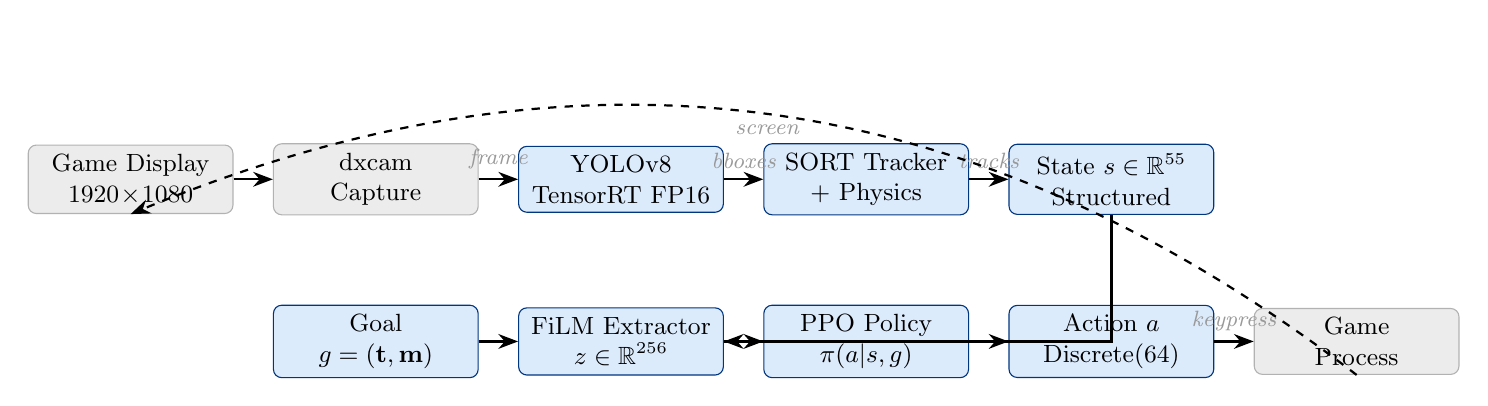
\begin{tikzpicture}[
    box/.style={rectangle, draw, rounded corners=3pt, minimum width=2.6cm, minimum height=0.8cm, align=center, font=\small},
    hwbox/.style={box, fill=gray!15, draw=gray!60},
    swbox/.style={box, fill=lightblue, draw=darkblue},
    arrow/.style={-{Stealth[length=2.5mm]}, thick},
    label/.style={font=\footnotesize\itshape, text=gray!80},
    node distance=0.4cm and 0.5cm
]
    % Hardware row
    \node[hwbox] (display) {Game Display\\$1920\!\times\!1080$};
    \node[hwbox, right=0.5cm of display] (dxcam) {dxcam\\Capture};
    \node[swbox, right=0.5cm of dxcam] (yolo) {YOLOv8\\TensorRT FP16};
    \node[swbox, right=0.5cm of yolo] (tracker) {SORT Tracker\\+ Physics};
    \node[swbox, right=0.5cm of tracker] (state) {State $s \in \mathbb{R}^{55}$\\Structured};

    % Bottom row: agent
    \node[swbox, below=1.2cm of yolo] (film) {FiLM Extractor\\$z \in \mathbb{R}^{256}$};
    \node[swbox, left=0.5cm of film] (goal) {Goal\\$g = (\mathbf{t}, \mathbf{m})$};
    \node[swbox, right=0.5cm of film] (ppo) {PPO Policy\\$\pi(a|s,g)$};
    \node[swbox, right=0.5cm of ppo] (action) {Action $a$\\Discrete(64)};
    \node[hwbox, right=0.5cm of action] (game) {Game\\Process};

    % Arrows top
    \draw[arrow] (display) -- (dxcam);
    \draw[arrow] (dxcam) -- (yolo) node[above, label, midway] {frame};
    \draw[arrow] (yolo) -- (tracker) node[above, label, midway] {bboxes};
    \draw[arrow] (tracker) -- (state) node[above, label, midway] {tracks};

    % State to agent
    \draw[arrow] (state) |- (film);
    \draw[arrow] (goal) -- (film);
    \draw[arrow] (film) -- (ppo);
    \draw[arrow] (ppo) -- (action);
    \draw[arrow] (action) -- (game) node[above, label, midway] {keypress};
    \draw[arrow, dashed, bend right=30] (game.south) to node[below, label] {screen} (display.south);
\end{tikzpicture}
\caption{End-to-end perception-to-action pipeline. Screen capture feeds YOLO detection, which is stabilized by a physics tracker to produce a structured 55-dim state. The FiLM extractor conditions the PPO policy on the current goal. Actions are sent to the live game process via keyboard simulation.}
\label{fig:pipeline}
\end{figure}

\subsection{Effective Throughput}

The full pipeline achieves approximately $37$--$41$ effective steps per second (measured: ${\sim}41$ steps/s in practice):
\begin{itemize}[leftmargin=1.5em]
    \item dxcam capture: $\sim$0 ms (non-blocking, asynchronous)
    \item YOLO TensorRT inference: $\sim$12--18 ms per frame
    \item Tracker + state update: $\sim$2 ms
    \item Policy forward pass: $\sim$3 ms
    \item Total: $\sim$18--25 ms per step $\Rightarrow$ $\sim$40--55 Hz, consistent with measured throughput.
\end{itemize}
YOLO inference runs every 2 steps; odd steps use physics-only prediction, halving GPU load without significant state quality degradation.

% ══════════════════════════════════════════════════════════════
\section{Failure Modes and Iterative Design}
\label{sec:failures}

We document four failed approaches chronologically.
Each failure's diagnosis directly motivated the next architectural decision.

\subsection{Attempt 1: Frame-Stacked Pixel Policy with Flat PPO}
\label{sec:pixel-failures}

\paragraph{Setup.}
End-to-end PPO from raw pixels: a 3-layer convolutional encoder processed $4$-frame stacks ($84 \times 84$ grayscale), feeding a 2-layer MLP policy and value head.
The reward combined stock changes, damage deltas, and a proximity bonus to the opponent.

\paragraph{Failure.}
The agent converged to trivial degenerate policies (constant idle, or oscillating movement) within $200$K frames.
No improvement was observed beyond $500$K frames on any random seed.

\paragraph{Diagnosis.}
\emph{Perceptual aliasing.}
The convolutional encoder could not distinguish states that were visually identical but mechanically distinct.
In Brawlhalla, the dominant pixel variance is from visual effects (knockback trails, damage flashes, background animations), not from the mechanically relevant features (damage percentage, weapon state, frame advantage).
The mapping $O: \mathcal{S} \to \Omega$ is not injective; no encoder can invert it.

\paragraph{Key insight.}
Game-relevant features (damage \%, weapon possession, proximity, grounding) occupy $<1\%$ of the pixel budget in a typical Brawlhalla frame.
The encoder was learning to represent visual noise, not game state.

\subsection{Attempt 2: Intrinsic Curiosity Augmentation}
\label{sec:curiosity-failure}

\paragraph{Hypothesis.}
Sparse extrinsic reward can be supplemented with intrinsic exploration bonuses~\cite{pathak2017curiosity}.

\paragraph{Setup.}
ICM-style intrinsic reward: a forward dynamics model in latent space generated prediction-error bonuses.
A separate inverse model trained alongside the encoder to predict actions from consecutive latent states.

\paragraph{Failure.}
The agent became ``curious'' about visually noisy states (explosions, knockback effects, particle-heavy animations) while ignoring strategically meaningful but visually simple states (positioning, approach, recovery).
Reward curves showed initial increase followed by stagnation.

\paragraph{Diagnosis.}
\emph{Curiosity is not aligned with strategic novelty.}
In high-entropy visual domains, prediction error in pixel space correlates with visual chaos, not with game-strategic novelty.
Death events---the worst possible game outcome---produce the most visually chaotic frames and were thus found ``maximally interesting'' by the curiosity module.
This created a perverse incentive to die repeatedly.

\subsection{Attempt 3: Pretrained ResNet-18 Encoder}
\label{sec:resnet-failure}

\paragraph{Hypothesis.}
Pretrained visual features (ImageNet-trained ResNet-18) provide better state discrimination than from-scratch CNNs.

\paragraph{Setup.}
Frozen ResNet-18 mapping $224 \times 224$ frames to $512$-dim embeddings; MLP policy on top.
The embedding was fine-tuned in a second stage with the policy.

\paragraph{Partial success.}
t-SNE visualization of the embeddings showed improved separation between game phases (neutral, combat, offstage).
The agent occasionally learned non-trivial movement patterns not observed with from-scratch CNN.

\paragraph{Failure.}
Training throughput fell to $2$--$5$ fps due to the ResNet forward pass on every step.
At this rate, collecting $500$K steps required $28$--$70$ hours wall-clock time per experiment, making iterative development impractical.
The agent still failed to learn coherent multi-phase behavior.

\paragraph{Diagnosis.}
\emph{Reward sparsity is orthogonal to state representation quality.}
Even with high-quality embeddings, if the reward signal arrives every $1000$--$5000$ frames, temporal credit assignment is intractable at $2$--$5$ fps throughput.
Better state encoding is necessary but not sufficient.

\subsection{Attempt 4: Flat Reward Shaping with YOLO State}
\label{sec:flat-reward-failure}

\paragraph{Breakthrough: YOLO for state extraction.}
Object detection reframes game-state extraction as a structured perception problem.
We fine-tuned YOLOv8 on annotated Brawlhalla frames to detect five classes:
\texttt{agent} (self), \texttt{op} (opponent unarmed), \texttt{op1}/\texttt{op2} (opponent with weapon types), and \texttt{weapons} (ground items).
This single detector simultaneously solves player identification, opponent localization, and weapon-state inference.
TensorRT conversion (FP16) reduced inference from $\sim$50 ms (PyTorch) to $\sim$15 ms, recovering the $3\times$ throughput loss from ResNet.

\paragraph{Failure.}
With structured 55-dim state, we designed a 9-component reward: damage dealt, KO bonuses, proximity, weapon possession, center control, edge penalty, dodge-use penalty, approach reward, and damage-ratio advantage.
The agent learned basic approach behavior but failed to chain sequential sub-objectives: it would not learn to \emph{first} pick up a weapon, \emph{then} approach, \emph{then} attack, because the flat reward provided no mechanism to prioritize temporally ordered sub-goals.

Gradients from contradictory reward components (e.g., ``approach opponent'' vs. ``stay on-stage'' when the opponent is near the edge) caused oscillating behavior that never committed to any coherent strategy.

\paragraph{Root cause.}
\emph{Sequential sub-objective structure cannot be expressed by a flat reward.}
This diagnosis motivated the transition to goal-conditioned hierarchical RL.

\begin{figure}[t]
\centering
\begin{tikzpicture}[
    attempt/.style={rectangle, draw, rounded corners=4pt, minimum width=3.8cm, minimum height=1.4cm, align=center, font=\small},
    failure/.style={attempt, fill=lightred!70, draw=darkred},
    success/.style={attempt, fill=lightgreen!70, draw=darkgreen},
    arrow/.style={-{Stealth[length=2.5mm]}, thick},
    ann/.style={font=\footnotesize\itshape, text=gray!70, align=center},
    node distance=0.3cm and 0.6cm
]
    \node[failure] (a1) {Attempt 1\\Pixel CNN + PPO\\{\tiny Perceptual aliasing}};
    \node[failure, right=0.5cm of a1] (a2) {Attempt 2\\+ Curiosity ICM\\{\tiny Noise ≠ novelty}};
    \node[failure, right=0.5cm of a2] (a3) {Attempt 3\\ResNet-18\\{\tiny Throughput crash}};
    \node[failure, right=0.5cm of a3] (a4) {Attempt 4\\YOLO + flat reward\\{\tiny Sequential failure}};
    \node[success, below=1.4cm of a2, xshift=3.2cm] (final) {\textbf{Final System}\\YOLO + FiLM-UVFA\\+ Curriculum + HSP};

    \draw[arrow, darkred] (a1) -- (a2) node[above, ann, midway] {add ICM};
    \draw[arrow, darkred] (a2) -- (a3) node[above, ann, midway] {better enc.};
    \draw[arrow, darkred] (a3) -- (a4) node[above, ann, midway] {YOLO};
    \draw[arrow, darkgreen, thick] (a4.south) -- ++(0,-0.5) -| (final.north) node[near start, ann, right] {goal-conditioned\\hierarchy};
\end{tikzpicture}
\caption{Iterative design trajectory. Each failed attempt reveals a specific, diagnosable failure mode that motivates the next architectural decision.}
\label{fig:trajectory}
\end{figure}

% ══════════════════════════════════════════════════════════════
\section{System Architecture}
\label{sec:architecture}

The failure analysis converges on three requirements: (1) structured object-centric state, (2) goal-conditioned dense reward, and (3) hierarchical temporal abstraction.
Figure~\ref{fig:architecture} shows the complete system.

\begin{figure}[t]
\centering
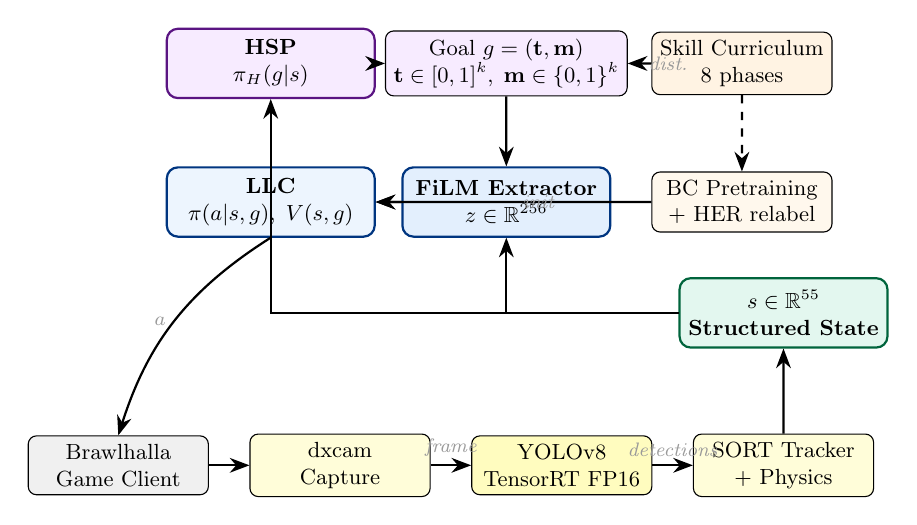
\begin{tikzpicture}[
    block/.style={rectangle, draw, rounded corners=3pt, minimum width=2.6cm, minimum height=0.85cm, align=center, font=\small},
    component/.style={rectangle, draw, thick, rounded corners=4pt, minimum width=3.0cm, minimum height=1.0cm, align=center, font=\small\bfseries},
    arrow/.style={-{Stealth[length=2.5mm]}, thick},
    darrow/.style={-{Stealth[length=2.5mm]}, thick, dashed},
    label/.style={font=\footnotesize\itshape, text=gray!80},
    scale=0.88, transform shape
]
    % Row 1 — Perception
    \node[block, fill=gray!12] (game) at (0, 0) {Brawlhalla\\Game Client};
    \node[block, fill=yellow!15] (cap) at (3.2, 0) {dxcam\\Capture};
    \node[block, fill=yellow!25] (yolo) at (6.4, 0) {YOLOv8\\TensorRT FP16};
    \node[block, fill=yellow!15] (track) at (9.6, 0) {SORT Tracker\\+ Physics};
    \node[component, fill=lightgreen!80, draw=darkgreen] (state) at (9.6, 2.2) {$s \in \mathbb{R}^{55}$\\Structured State};

    % Row 2 — LLC
    \node[component, fill=lightblue!80, draw=darkblue] (film) at (5.6, 3.8) {FiLM Extractor\\$z \in \mathbb{R}^{256}$};
    \node[component, fill=lightblue!50, draw=darkblue] (llc) at (2.2, 3.8) {LLC\\$\pi(a|s,g),\;V(s,g)$};
    \node[block, fill=lightpurple!80] (goal) at (5.6, 5.8) {Goal $g = (\mathbf{t}, \mathbf{m})$\\$\mathbf{t} \in [0,1]^k,\;\mathbf{m} \in \{0,1\}^k$};

    % Row 3 — HSP + Curriculum
    \node[component, fill=lightpurple!80, draw=darkpurple] (hsp) at (2.2, 5.8) {HSP\\$\pi_H(g|s)$};
    \node[block, fill=lightorange!80] (curriculum) at (9.0, 5.8) {Skill Curriculum\\8 phases};
    \node[block, fill=lightorange!50] (bc) at (9.0, 3.8) {BC Pretraining\\+ HER relabel};

    % Arrows
    \draw[arrow] (game) -- (cap);
    \draw[arrow] (cap) -- (yolo) node[above, label, midway] {frame};
    \draw[arrow] (yolo) -- (track) node[above, label, midway] {detections};
    \draw[arrow] (track) -- (state);
    \draw[arrow] (state) -| (film);
    \draw[arrow] (state) -| (hsp);
    \draw[arrow] (hsp) -- (goal);
    \draw[arrow] (goal) -- (film);
    \draw[arrow] (film) -- (llc);
    \draw[arrow] (curriculum) -- (goal) node[right, label, midway] {dist.};
    \draw[arrow] (bc) -- (llc) node[right, label, midway] {init};
    \draw[arrow, bend right=20] (llc.south) to node[left, label] {$a$} (game.north);
    \draw[darrow] (curriculum) -- (bc);
\end{tikzpicture}
\caption{Complete system architecture. YOLO extracts object-centric bounding boxes; a physics tracker produces a consistent 55-dim state. The skill curriculum defines goal distributions; behavioral cloning warm-starts the LLC. The FiLM extractor conditions the LLC on the current goal. The HSP selects goals at macro-timescale; the LLC executes motor primitives.}
\label{fig:architecture}
\end{figure}

The system decomposes into three major components, each resolving one failure mode:
\begin{enumerate}[leftmargin=1.5em]
    \item \textbf{Structured Perception} (Section~\ref{sec:state-representation}): YOLO + tracker resolve perceptual aliasing.
    \item \textbf{Goal-Conditioned LLC} (Sections~\ref{sec:llc}--\ref{sec:curriculum}): UVFA + curriculum resolve reward sparsity and behavioral complexity.
    \item \textbf{Strategic Planner} (Section~\ref{sec:hsp}): HSP resolves sequential sub-objective composition at match timescale.
\end{enumerate}

% ══════════════════════════════════════════════════════════════
\section{State Representation}
\label{sec:state-representation}

\subsection{Object Detection via Fine-Tuned YOLOv8}
\label{sec:yolo}

The core perceptual breakthrough is treating game-state extraction as an object detection task.
We fine-tuned YOLOv8~\cite{jocher2023yolov8} on a dataset of annotated Brawlhalla frames covering five object classes:

\begin{table}[h]
\centering
\small
\begin{tabular}{@{}lll@{}}
\toprule
\textbf{Class} & \textbf{Meaning} & \textbf{Information Provided} \\
\midrule
\texttt{agent} & Controlled player & Self-position, size, facing \\
\texttt{op} & Opponent (unarmed) & Opponent position, unarmed state \\
\texttt{op1} & Opponent (weapon type A) & Opponent position + weapon state \\
\texttt{op2} & Opponent (weapon type B) & Opponent position + weapon state \\
\texttt{weapons} & Ground weapon item & Weapon position, pickup opportunity \\
\bottomrule
\end{tabular}
\caption{YOLO detection classes. Opponent weapon possession is inferred from the class label in a single forward pass.}
\end{table}

This design choice is notable: rather than running a separate weapon-state classifier, the class label itself encodes weapon possession.
A single forward pass simultaneously localizes all game-relevant objects and infers their semantic state.

For inference speed, the PyTorch YOLOv8 model is converted to a TensorRT engine (\texttt{best.engine}) with FP16 precision.
This reduces inference latency by ${\sim}3\times$ ($50$ ms $\to$ $15$ ms), recovering the throughput budget needed for learning.

\subsection{Physics-Based Tracking and State Memory}
\label{sec:tracker}

Raw YOLO detections are bounding boxes: they have jitter, missed frames, and no temporal identity assignment.
A SORT-like tracker~\cite{bewley2016simple} resolves this through IoU-based Hungarian matching, maintaining persistent track IDs across frames.
Per-object velocities are estimated from two-frame position differences.

Detected positions are fused with constant-velocity physics predictions via exponential smoothing:
\begin{equation}
\hat{p}_t = \alpha \cdot p_t^{\text{YOLO}} + (1 - \alpha) \cdot \hat{p}_{t-1}^{\text{physics}}, \quad \alpha = 0.85
\label{eq:position-fusion}
\end{equation}

On frames where YOLO does not run (every other frame), the physics prediction $\hat{p}_t^{\text{physics}} = \hat{p}_{t-1} + v_{t-1} \cdot \Delta t$ is used directly, maintaining smooth state estimates at half the YOLO inference cost.

\subsection{Structured State Vector $s \in \mathbb{R}^{55}$}

The tracker output and HUD pixel readings are assembled into a 55-dimensional observation vector.
The state is organized into feature groups:

\begin{table}[t]
\centering
\caption{Structured state vector $s \in \mathbb{R}^{55}$. All features are normalized to $[0,1]$ or $[-1,1]$.}
\label{tab:state-spec}
\small
\begin{tabular}{@{}llcl@{}}
\toprule
\textbf{Group} & \textbf{Features} & \textbf{Dim} & \textbf{Range} \\
\midrule
Player kinematics & $x, y, v_x, v_y$, grounded, dmg\%, weapon, jumps, edge, offstage & 10 & $[0,1]$ / $[-1,1]$ \\
Opponent kinematics & Mirrored player features & 10 & $[0,1]$ / $[-1,1]$ \\
Relational geometry & $\Delta x, \Delta y, d$, strike-range, facing, facing-dir, weapon $\Delta x / \Delta y$ & 8 & $[-1,1]$ / $[0,2]$ \\
Game state & Stocks (self/opp), dodge cooldown, weapon-on-ground & 4 & $[0,1]$ \\
Recovery & Ledge distance, signed $\Delta x/\Delta y$ to ledge & 3 & $[0,2]$ / $[-1,1]$ \\
Temporal/strategic & Airborne time (self/opp), hitstun (self/opp) & 4 & $[0,1]$ \\
Combat extended & opp-facing, time-since-hit, knockback, center-dist, + & 12 & various \\
Previous action & Movement, jump, dodge, attack (normalized) & 4 & $[0,1]$ \\
\midrule
\textbf{Total} & & \textbf{55} & \\
\bottomrule
\end{tabular}
\end{table}

\subsection{Damage Estimation from HUD Pixels}

Brawlhalla provides no programmatic access to damage percentages.
We extract damage by reading fixed-position HUD regions and mapping their dominant color to damage via a hand-calibrated 9-stage gradient function:
\begin{equation}
d_{\text{pct}} = f_{\text{color}}(r, g, b) \in [0, 1],
\quad f_{\text{color}}: \texttt{white} \to \texttt{yellow} \to \texttt{orange} \to \texttt{red} \to \texttt{black}
\end{equation}
corresponding to the $0 \to 350$\% damage progression.
Stock events (loss, gain) are detected via red/cyan flash pixels in the stock-display HUD regions.

This approach requires zero game API access and adds negligible latency ($< 1$ ms), at the cost of requiring fixed screen positions and tuned color thresholds.

% ══════════════════════════════════════════════════════════════
\section{Goal-Conditioned Low-Level Controller}
\label{sec:llc}

\subsection{Goal-Conditioned MDP Formulation}

We replace the original Brawlhalla POMDP with a structured goal-conditioned MDP over the extracted state representation.

\begin{definition}[Goal-Conditioned MDP]
$\mathcal{M}_g = (\mathcal{S}, \mathcal{A}, \mathcal{G}, P, r_g, \gamma)$ where $\mathcal{S} = \mathbb{R}^{55}$, $\mathcal{A} = \text{Discrete}(64)$ (flattened MultiDiscrete), $\mathcal{G}$ is the structured goal space (Definition~\ref{def:masked-goal}), and $r_g$ is the masked MAE goal-progress reward (Section~\ref{sec:reward}).
\end{definition}

\subsection{Factored Goal Representation}
\label{sec:structured-goals}

\begin{definition}[Factored Goal]
\label{def:masked-goal}
A goal is a composite structure $g = (g_{\text{type}},\, \tilde{g})$ where $g_{\text{type}} \in \mathcal{T}$ is a discrete goal type selected from the finite set
\[
\mathcal{T} = \{\texttt{recovery},\; \texttt{approach},\; \texttt{spacing},\; \texttt{attack},\; \texttt{weapon}\},
\]
and $\tilde{g} \in \mathbb{R}^{d_{g_{\text{type}}}}$ is a type-specific continuous parameter vector.
The binary feature mask $\mathbf{m} = \text{mask}(g_{\text{type}}) \in \{0,1\}^k$ is derived \emph{deterministically} from $g_{\text{type}}$, and the target projection $\mathbf{t} \in [0,1]^k$ is constructed from $\tilde{g}$.
The full masked goal vector is:
\begin{equation}
g_{\text{full}} = \text{mask}(g_{\text{type}}) \odot \mathbf{t}(g_{\text{type}},\, \tilde{g}) \in [0,1]^k
\label{eq:factored-goal}
\end{equation}
\end{definition}

This \emph{factored} representation supersedes the naive target-mask pair $(\mathbf{t}, \mathbf{m})$: the mask is no longer a free binary input to be predicted or provided arbitrarily, but is \emph{determined} by the goal type, making the goal space semantically typed and structured.
The FiLM generator receives the goal type (as a one-hot $\mathbf{1}_{g_{\text{type}}} \in \mathbb{R}^{|\mathcal{T}|}$) alongside the derived $(g_{\text{full}},\, \mathbf{m})$, enabling type-conditioned modulation while sharing all parameters across goal types.

Our implementation uses $k = 10$ curriculum goal features:
\begin{equation}
f(s) = \bigl[x_p,\; y_p,\; \mathbb{1}_{\text{weapon}},\; w_{\Delta x},\; w_{\Delta y},\; \mathbb{1}_{\text{strike}},\; d_{\text{opp}},\; \phi_{\text{facing}},\; \Delta_{\text{frame}},\; \mathbb{1}_{\text{offstage}}\bigr]
\label{eq:goal-features}
\end{equation}

Table~\ref{tab:goal-types} specifies the semantic parameter vector $\tilde{g}$ and the derived mask for each type.

\begin{table}[h]
\centering
\small
\caption{Factored goal type definitions. The mask $\mathbf{m}$ is derived deterministically from $g_{\text{type}}$; $\tilde{g}$ are the type-specific semantic parameters.}
\label{tab:goal-types}
\begin{tabular}{@{}llll@{}}
\toprule
\textbf{Goal Type} & \textbf{Parameters $\tilde{g}$} & \textbf{Active Mask Dims} & \textbf{Tactical Intent} \\
\midrule
\texttt{recovery} & $(\text{target}\_x,\; \text{target}\_y,\; \text{urgency})$ & $x_p,\; y_p,\; \mathbb{1}_{\text{offstage}}$ & Return to platform \\
\texttt{approach} & $(\text{rel\_dist},\; \text{vert\_align},\; \text{facing\_req})$ & $x_p,\; d_{\text{opp}},\; \phi_{\text{facing}}$ & Close distance to opponent \\
\texttt{spacing} & $(\text{desired\_dist},\; \text{direction})$ & $d_{\text{opp}},\; \mathbb{1}_{\text{strike}},\; \Delta_{\text{frame}}$ & Maintain frame advantage \\
\texttt{attack} & $(\text{in\_range},\; \text{atk\_type},\; \text{opp\_state})$ & $\mathbb{1}_{\text{strike}},\; d_{\text{opp}},\; \Delta_{\text{frame}}$ & Enter strike range \\
\texttt{weapon} & $(\text{wpn}\_\Delta x,\; \text{wpn}\_\Delta y,\; \text{pickup\_flag})$ & $w_{\Delta x},\; w_{\Delta y},\; \mathbb{1}_{\text{weapon}}$ & Pick up weapon \\
\bottomrule
\end{tabular}
\end{table}

\begin{remark}[Why typed partial masking is essential]
Consider a \texttt{recovery} goal: the agent must return to platform, making opponent distance and frame advantage entirely irrelevant.
Including those dimensions in the error signal injects spurious gradients.
By making the mask a \emph{deterministic function of the goal type}, we guarantee that the policy gradient is semantically meaningful at every step---each active dimension corresponds to a feature that definitionally matters for the current tactical intent.
Simultaneously, sharing parameters across types allows motor primitives learned in recovery to transfer to approach, spacing, and attack without any re-parameterization.
\end{remark}

\subsection{Goal Sampling Distribution}
\label{sec:goal-sampling}

Online goals are drawn from a composite distribution that mixes three sources:
\begin{equation}
P(g) = 0.4\, G_{\text{core}} + 0.4\, G_{\text{HER}} + 0.2\, G_{\text{archive}}
\label{eq:goal-sampling}
\end{equation}

\begin{itemize}[leftmargin=1.5em]
    \item $G_{\text{core}}$: the phase-specific \texttt{TargetSampler}, drawing targets from tactically meaningful configurations (e.g., platform bounds for locomotion, opponent proximity ranges for combat).
    \item $G_{\text{HER}}$: hindsight goals generated from future states in the \emph{current} episode; achieved feature vectors become goal targets, converting every trajectory into goal-conditioned training signal.
    \item $G_{\text{archive}}$: goals sampled from successful trajectories stored in the replay buffer, providing behavioral anchors to previously mastered skills.
\end{itemize}

\paragraph{Temporal consistency.}
Goals are held constant for a fixed horizon before resampling:
\begin{equation}
g_t = g_{t+1} = \cdots = g_{t+k}, \quad k \sim \mathcal{U}(16, 32)
\label{eq:goal-temporal}
\end{equation}
A minimum of $k_{\min} = 16$ steps is enforced to prevent rapid cycling that would allow the policy to exploit short-duration goal-achievement bonuses.

\begin{proposition}[Reduced effective goal dimensionality]
\label{prop:dim-reduction}
With $k$ goal features and $\ell$ active mask dimensions ($\ell \ll k$ in practice), the effective goal manifold has dimension $\ell$, not $k$.
The UVFA generalization error $\epsilon_{\text{gen}}$ scales with the effective dimensionality $\ell$~\cite{schaul2015universal}, not the nominal dimensionality $k$.
\end{proposition}

\begin{proof}[Sketch]
Goals with the same active set $\mathcal{I} = \{i : m_i = 1\}$ form a $|\mathcal{I}|$-dimensional submanifold of $[0,1]^k$.
The value function $V(s, g)$ varies only along the $|\mathcal{I}|$ active dimensions within each submanifold.
For a given active set, the sample complexity of learning $V$ to $\epsilon$ accuracy is polynomial in $|\mathcal{I}|$ rather than $k$.
\end{proof}

In our system, $k = 10$ but typical goals activate $\ell = 2$--$4$ dimensions, yielding a $2.5$--$5\times$ effective complexity reduction.

\subsection{Goal Error and Reward Function}
\label{sec:reward}

\begin{definition}[Masked Goal Error]
The instantaneous goal error is the masked mean absolute error (MAE):
\begin{equation}
\varepsilon(s, g) = \sum_{i=1}^{k} m_i \cdot |f_i(s) - t_i|
\label{eq:goal-error}
\end{equation}
\end{definition}

The LLC reward is a potential-based shaping term plus sparse events:

\begin{equation}
\boxed{
r(s_t, a_t, g) = \underbrace{\text{clip}\bigl(\lambda_p \cdot [\varepsilon(s_t, g) - \varepsilon(s_{t+1}, g)],\; r_{\min},\; r_{\max}\bigr)}_{\text{dense goal progress}} + \underbrace{r_{\text{sparse}}(s_t, s_{t+1})}_{\text{terminal events}}
}
\label{eq:llc-reward}
\end{equation}

where $\lambda_p = 5.0$, $r_{\min} = -0.1$, $r_{\max} = 0.3$, and:

\begin{equation}
r_{\text{sparse}} = \begin{cases}
    +r_{\text{success}} & \text{if } \varepsilon(s_{t+1}, g) < \varepsilon_{\text{thresh}} \\[3pt]
    -r_{\text{death}} & \text{if player loses a stock} \\[3pt]
    +r_{\text{hit}} \cdot \Delta d_{\text{opp}} & \text{if opponent damage increases} \\[3pt]
    0 & \text{otherwise}
\end{cases}
\end{equation}

\begin{proposition}[Shaping consistency]
\label{prop:shaping}
The dense component $F_t = \varepsilon(s_t, g) - \varepsilon(s_{t+1}, g)$ is a valid potential-based shaping function~\cite{ng1999policy} with potential $\Phi(s, g) = -\varepsilon(s, g)$.
Any policy that is optimal under the shaped reward $r + F$ is also optimal under the base sparse reward $r$.
\end{proposition}

\begin{proof}
By~\cite{ng1999policy}, $F(s, s', g) = \gamma \Phi(s', g) - \Phi(s, g)$ with $\Phi(s, g) = -\varepsilon(s, g)$ is a valid shaping function for any $\gamma \in [0, 1)$.
In our case $F_t \approx \varepsilon(s_t, g) - \varepsilon(s_{t+1}, g)$ (the $\gamma$-discounted version approximated at $\gamma \approx 1$).
The clipping introduces a bounded approximation: $|F_t - F_t^{\text{exact}}| \leq |r_{\max}|/\lambda_p$ uniformly, which vanishes as $r_{\max} \to \infty$.
\end{proof}

The critical property of this reward: \emph{every single frame produces a non-zero gradient signal} as long as the goal error is changing.
This converts the sparse reward problem into a dense regression problem, the same effect as HER but without requiring off-policy data.

\subsection{Universal Value Function Approximation}
\label{sec:uvfa}

\begin{definition}[UVFA~\cite{schaul2015universal}]
A Universal Value Function Approximator is a single parameterized function family $V_\phi(s, g)$ that simultaneously approximates $V^*(s, g)$ for all $(s, g) \in \mathcal{S} \times \mathcal{G}$.
\end{definition}

The LLC is trained as an actor-critic UVFA: a shared FiLM feature extractor feeds separate policy and value heads, both conditioned on the current goal $g$.
The augmented observation is:
\begin{equation}
\tilde{s} = [s;\; \tilde{e};\; \mathbf{m};\; \alpha;\; \mathbf{1}_{g_{\text{type}}}] \in \mathbb{R}^{55 + 3k + |\mathcal{T}|}
\label{eq:augmented-obs}
\end{equation}
where $\tilde{e}$ is the masked goal error, $\mathbf{m}$ is the type-derived mask, $\alpha$ is the goal-alignment signal (Section~\ref{sec:film}), and $\mathbf{1}_{g_{\text{type}}} \in \mathbb{R}^5$ is the one-hot goal-type encoding.
PPO trains both $\pi_\theta(a | \tilde{s})$ and $V_\phi(\tilde{s})$ where $g$ is fully embedded inside $\tilde{s}$.

\subsection{Hindsight Goal Relabeling for BC Pretraining}
\label{sec:her}

Hindsight Experience Replay~\cite{andrychowicz2017hindsight} is incompatible with on-policy PPO because it requires re-weighting transitions under a different goal.
We instead apply HER-style relabeling at the \emph{behavioral cloning pretraining} stage:

For each demonstration transition $(s_t, a_t)$, we generate hindsight goal-conditioned training tuples:
\begin{equation}
\{(s_t,\; g_{t+h},\; a_t) \;:\; h \in \{1, 2, 4, 8\}\}, \quad g_{t+h} = f(s_{t+h})
\end{equation}

This produces $4\times$ more training data from the same demonstration, spanning a rich distribution of goal-conditioned behaviors.
PPO then fine-tunes from this initialization, with the potential-based reward providing dense signal throughout.

% ══════════════════════════════════════════════════════════════
\section{FiLM-Based Goal Modulation}
\label{sec:film}

\subsection{Motivation}

Naive concatenation $[s; \mathbf{t}; \mathbf{m}]$ into a flat MLP provides no structural information about the \emph{role} of goal information.
The network must discover from scratch that goals are contextual modifiers of behavior, not additional state features.
In practice, concatenation-based policies exhibited slower goal-adaptation speed and sharper performance degradation when goal distributions shifted between curriculum phases.

Feature-wise Linear Modulation (FiLM)~\cite{perez2018film} resolves this by using goal information to generate \emph{affine transform parameters} that modulate state feature maps.
This creates an architectural inductive bias: goals specify \emph{how to process} state, not \emph{what to observe}.

\subsection{Architecture in Detail}
\label{sec:film-arch}

The FiLM extractor operates in four stages.
Let $s \in \mathbb{R}^{55}$, $\mathbf{t} \in [0,1]^k$, $\mathbf{m} \in \{0,1\}^k$.

\paragraph{Stage 1: State augmentation.}
Extract goal-relevant features and compute auxiliary signals:
\begin{align}
\hat{f}_i &= \text{clip}\!\left(\frac{f_i(s) - \ell_i}{u_i - \ell_i},\; 0,\; 1\right) \quad \text{(normalized features)} \label{eq:norm-feats} \\
e_i &= \hat{f}_i - t_i \in [-1, 1] \quad \text{(goal error per dimension)} \label{eq:goal-error-vec} \\
\tilde{e}_i &= m_i \cdot e_i \quad \text{(masked error)} \label{eq:masked-error} \\
v_{\text{speed}} &= \tanh\!\bigl(\sqrt{v_x^2 + v_y^2}\bigr) \label{eq:speed} \\
\alpha_i &= m_i \cdot \text{sign}(e_i) \cdot v_{\text{speed}} \in [-1, 1] \quad \text{(goal alignment)} \label{eq:goal-alignment}
\end{align}

The goal-alignment signal $\alpha$ encodes ``am I currently moving toward or away from each active goal dimension, and at what speed?''
This provides a direct motor-outcome-goal progress coupling that dramatically accelerates early training.

Augmented state:
\begin{equation}
s_{\text{aug}} = [s;\; \tilde{e};\; \mathbf{m};\; \alpha] \in \mathbb{R}^{55 + 3k}
\end{equation}

\paragraph{Stage 2: Dual encoding.}
\begin{align}
\phi(s) &= \text{MLP}_{\text{state}}(s_{\text{aug}}) \in \mathbb{R}^{256} \label{eq:state-enc} \\
\psi(g) &= \text{MLP}_{\text{goal}}([\mathbf{t};\; \mathbf{m}]) \in \mathbb{R}^{128} \label{eq:goal-enc}
\end{align}
Both MLPs use 2 hidden layers with ReLU activations.

\paragraph{Stage 3: FiLM modulation with residual.}
\begin{align}
[\gamma;\; \beta] &= W_{\text{FiLM}} \psi(g) + b_{\text{FiLM}}, \quad \gamma, \beta \in \mathbb{R}^{256} \label{eq:film-params} \\
h &= \underbrace{\gamma \odot \phi(s) + \beta}_{\text{modulated}} + \underbrace{\phi(s)}_{\text{residual}} \label{eq:film-modulation}
\end{align}

The gamma parameters are clamped: $\gamma \in [0.5, 1.5]$.
The beta parameters are clamped: $\beta \in [-1.0, 1.0]$.
These clamps prevent gradient blow-up during early training while allowing meaningful modulation range.
The residual connection $+\phi(s)$ guarantees the network is always at least as expressive as a goal-independent policy.

\paragraph{Stage 4: Post-modulation.}
\begin{equation}
z = \text{MLP}_{\text{post}}(\text{ReLU}(h)) \in \mathbb{R}^{256}
\end{equation}
$z$ is the extractor output fed into the PPO policy and value heads.

\begin{figure}[t]
\centering
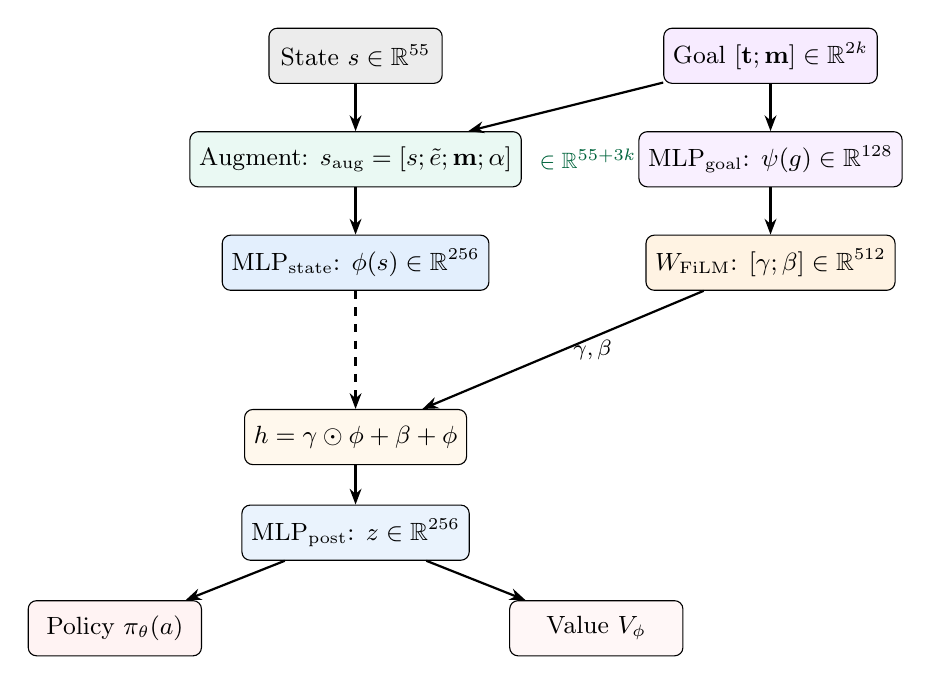
\begin{tikzpicture}[
    mbox/.style={rectangle, draw, rounded corners=3pt, minimum width=2.2cm, minimum height=0.7cm, align=center, font=\small},
    op/.style={circle, draw, minimum size=0.5cm, font=\footnotesize},
    arrow/.style={-{Stealth[length=2mm]}, thick},
    node distance=0.35cm and 0.5cm
]
    % Inputs
    \node[mbox, fill=gray!15] (s) {State $s \in \mathbb{R}^{55}$};
    \node[mbox, fill=lightpurple!80, right=2.8cm of s] (g) {Goal $[\mathbf{t};\mathbf{m}] \in \mathbb{R}^{2k}$};

    % Augmentation
    \node[mbox, fill=lightgreen!60, below=0.6cm of s] (aug) {Augment: $s_{\text{aug}} = [s;\tilde{e};\mathbf{m};\alpha]$};
    \node[font=\footnotesize\itshape, right=0.1cm of aug, text=darkgreen] {$\in \mathbb{R}^{55+3k}$};

    % Encoders
    \node[mbox, fill=lightblue!80, below=0.6cm of aug] (phi) {$\text{MLP}_{\text{state}}$: $\phi(s) \in \mathbb{R}^{256}$};
    \node[mbox, fill=lightpurple!60, below=0.6cm of g] (psi) {$\text{MLP}_{\text{goal}}$: $\psi(g) \in \mathbb{R}^{128}$};

    % FiLM generator
    \node[mbox, fill=lightorange!80, below=0.6cm of psi] (film) {$W_{\text{FiLM}}$: $[\gamma; \beta] \in \mathbb{R}^{512}$};

    % FiLM op
    \node[mbox, fill=lightorange!50, below=1.5cm of phi] (filmop) {$h = \gamma \odot \phi + \beta + \phi$};

    % Post
    \node[mbox, fill=lightblue!60, below=0.5cm of filmop] (post) {$\text{MLP}_{\text{post}}$: $z \in \mathbb{R}^{256}$};

    % Heads
    \node[mbox, fill=lightred!60, below left=0.5cm and 0.5cm of post] (pi) {Policy $\pi_\theta(a)$};
    \node[mbox, fill=lightred!40, below right=0.5cm and 0.5cm of post] (v) {Value $V_\phi$};

    % Arrows
    \draw[arrow] (s) -- (aug);
    \draw[arrow] (g) -- (aug);
    \draw[arrow] (aug) -- (phi);
    \draw[arrow] (g) -- (psi);
    \draw[arrow] (psi) -- (film);
    \draw[arrow, dashed] (phi) -- (filmop);
    \draw[arrow] (film) -- (filmop) node[right, font=\footnotesize\itshape, midway] {$\gamma, \beta$};
    \draw[arrow] (filmop) -- (post);
    \draw[arrow] (post) -- (pi);
    \draw[arrow] (post) -- (v);
\end{tikzpicture}
\caption{FiLM extractor architecture. The goal generates affine parameters $(\gamma, \beta)$ that modulate the state encoding via element-wise scaling and shifting plus a residual connection. Policy and value heads share the extractor.}
\label{fig:film}
\end{figure}

\subsection{FiLM as Conditional Computation}

FiLM modulation instantiates a family of linear operators parametrized by the goal:
\begin{equation}
h(s, g) = \underbrace{(\mathbf{I} + \text{diag}(\gamma(g)))}_{\text{goal-conditioned scale}} \cdot \phi(s) + \beta(g)
\end{equation}
This is a first-order Taylor approximation to arbitrary goal-conditioned nonlinear operators, exact in the limit of many FiLM layers.
The residual ensures that $h = \phi(s)$ when $\gamma = 0, \beta = 0$, providing a smooth interpolation between goal-agnostic and goal-specific processing.

Compared to alternatives:
\begin{itemize}[leftmargin=1.5em]
    \item \textbf{Concatenation}: no structural inductive bias; slower goal adaptation in practice.
    \item \textbf{Discrete skill heads}: hard partitions prevent cross-goal gradient sharing; locomotion knowledge from recovery does not transfer to approach.
    \item \textbf{Hypernetworks}: more expressive but $10\times$ more parameters and high variance; FiLM's $66$K parameters (for the FiLM layer) are sufficient for our goal dimensionality.
\end{itemize}

% ══════════════════════════════════════════════════════════════
\section{Skill Curriculum}
\label{sec:curriculum}

\subsection{Curriculum Design Philosophy}

The curriculum embeds three domain-specific pedagogical principles:

\begin{enumerate}[leftmargin=1.5em]
    \item \textbf{Motor before strategy}: master spatial locomotion before engaging in combat. An agent that cannot reliably move to a target cannot benefit from combat training.
    \item \textbf{Constrained before free}: begin with action masking (no combat actions) to isolate the learning problem. Remove constraints progressively as competence is demonstrated.
    \item \textbf{Static before dynamic}: train against a non-responsive environment (empty arena) before introducing an opponent.
\end{enumerate}

The curriculum also serves as a \emph{reward decomposition}: instead of one complex reward for winning the game, each phase has a single, simple reward objective that is achievable within the phase's timestep budget.

\subsection{Eight Training Phases}

Each phase is defined by a \texttt{StageSpec} specifying: active goal mask, goal target sampler, action mask, and reward coefficients.
Table~\ref{tab:curriculum} documents all eight phases.

\begin{table}[t]
\centering
\caption{Eight-phase LLC training curriculum. Each phase introduces new skill complexity and warm-starts from the previous phase's weights.}
\label{tab:curriculum}
\small
\begin{tabular}{@{}clp{3.0cm}p{2.5cm}p{3.2cm}@{}}
\toprule
\textbf{\#} & \textbf{Phase Name} & \textbf{Active Goal Dims} & \textbf{Action Mask} & \textbf{Reward Focus} \\
\midrule
1 & \texttt{locomotion\_grounded} & $x_p, y_p$ & No jump, no attack & MAE progress + step cost \\
2 & \texttt{locomotion\_airborne} & $x_p, y_p$ & No attack & + jump usage \\
3 & \texttt{locomotion\_recovery} & $x_p, y_p, \mathbb{1}_{\text{offstage}}$ & Dodge enabled & + offstage penalty \\
4 & \texttt{locomotion} & $x_p, y_p, \mathbb{1}_{\text{offstage}}$ & Full movement & Combined locomotion \\
5 & \texttt{weapon\_control} & $w_{\Delta x}, w_{\Delta y}, \mathbb{1}_{\text{weapon}}$ & Full & Weapon acquisition bonus \\
6 & \texttt{damage\_static\_fist} & 6D combat goal & Full & Damage dealt (unarmed) \\
7 & \texttt{damage\_static\_weapon} & 6D combat goal & Full & Damage dealt $\times 2$ \\
8 & \texttt{damage\_dynamic} & Full 10D goal & Full & Damage dealt $\times 2.5$ \\
\bottomrule
\end{tabular}
\end{table}

\begin{figure}[t]
\centering
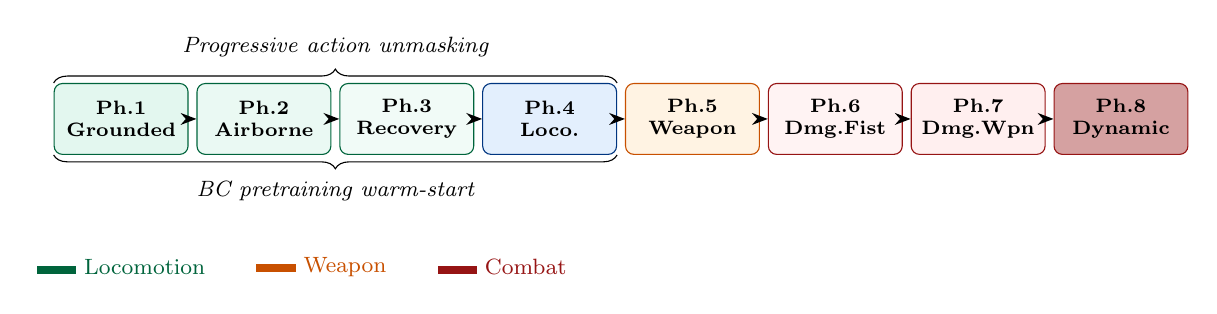
\begin{tikzpicture}[
    phase/.style={rectangle, draw, rounded corners=3pt, minimum width=1.7cm, minimum height=0.9cm, align=center, font=\scriptsize\bfseries},
    arrow/.style={-{Stealth[length=2mm]}, thick},
    node distance=0.15cm and 0.0cm
]
    % Phase boxes
    \node[phase, fill=lightgreen!80, draw=darkgreen] (p1) {Ph.1\\Grounded};
    \node[phase, fill=lightgreen!60, draw=darkgreen, right=0.1cm of p1] (p2) {Ph.2\\Airborne};
    \node[phase, fill=lightgreen!40, draw=darkgreen, right=0.1cm of p2] (p3) {Ph.3\\Recovery};
    \node[phase, fill=lightblue!80, draw=darkblue, right=0.1cm of p3] (p4) {Ph.4\\Loco.};
    \node[phase, fill=lightorange!80, draw=darkorange, right=0.1cm of p4] (p5) {Ph.5\\Weapon};
    \node[phase, fill=lightred!60, draw=darkred, right=0.1cm of p5] (p6) {Ph.6\\Dmg.Fist};
    \node[phase, fill=lightred!80, draw=darkred, right=0.1cm of p6] (p7) {Ph.7\\Dmg.Wpn};
    \node[phase, fill=darkred!40, draw=darkred, right=0.1cm of p7] (p8) {Ph.8\\Dynamic};

    % Arrows between phases
    \foreach \a/\b in {p1/p2, p2/p3, p3/p4, p4/p5, p5/p6, p6/p7, p7/p8} {
        \draw[arrow] (\a.east) -- (\b.west);
    }

    % BC annotation
    \draw[decorate, decoration={brace, amplitude=5pt, mirror}] (p1.south west) -- (p4.south east)
        node[midway, below=6pt, font=\footnotesize\itshape] {BC pretraining warm-start};

    % Action mask annotation
    \draw[decorate, decoration={brace, amplitude=5pt}] (p1.north west) -- (p4.north east)
        node[midway, above=6pt, font=\footnotesize\itshape] {Progressive action unmasking};

    % Color legend
    \node[font=\footnotesize, below=1.2cm of p1, text=darkgreen] (l1) {\rule{0.5cm}{3pt} Locomotion};
    \node[font=\footnotesize, right=0.4cm of l1, text=darkorange] (l2) {\rule{0.5cm}{3pt} Weapon};
    \node[font=\footnotesize, right=0.4cm of l2, text=darkred] (l3) {\rule{0.5cm}{3pt} Combat};
\end{tikzpicture}
\caption{Eight-phase curriculum progression. Each phase warm-starts from the previous. Locomotion phases use action masking (no combat actions) and BC pretraining initialization. Progressive unmasking and complexity increase follow the natural skill dependency graph.}
\label{fig:curriculum}
\end{figure}

\subsection{Phase Transitions and Weight Transfer}

Each phase is trained for a fixed budget (typically $500$K--$1$M timesteps).
At phase transition, the full model weights transfer: both the FiLM extractor and the PPO policy/value heads.
The FiLM architecture facilitates transfer particularly well: the shared motor backbone (state encoder + post-FiLM MLP) transfers motor primitives, while the goal encoder and FiLM generator adapt to the new goal distribution.

\subsection{Behavioral Cloning Pretraining}

Before Phase 1 PPO training, the LLC is initialized via behavioral cloning on human keyboard demonstrations.
The BC loss is cross-entropy over the discrete action space:
\begin{equation}
\mathcal{L}_{\text{BC}} = -\mathbb{E}_{(s, g, a) \sim \mathcal{D}_{\text{demo}}} \left[\log \pi_\theta(a \mid \tilde{s}(s, g))\right]
\label{eq:bc-loss}
\end{equation}
Demonstrations are augmented with HER relabeling at horizons $h \in \{1, 2, 4, 8\}$ (Section~\ref{sec:her}).

This initialization avoids the random-walk exploration problem in the early phases: a policy initialized with human locomotion behavior immediately begins making goal-directed progress, producing meaningful rewards from the first training step.

% ══════════════════════════════════════════════════════════════
\section{Anchored-Replay Proximal Policy Optimization}
\label{sec:ppo}

Standard PPO~\cite{schulman2017proximal} is the base optimizer for the LLC.
However, the curriculum setting creates challenges that motivate several extensions.
We implement a custom \texttt{AnchoredReplayPPO} optimizer with four modifications.

\subsection{Standard PPO}

The PPO objective clips the policy ratio to prevent destructive large updates:
\begin{equation}
\mathcal{L}^{\text{CLIP}}(\theta) = \mathbb{E}_t\!\left[\min\!\left(r_t(\theta) \hat{A}_t,\; \text{clip}(r_t(\theta), 1-\epsilon, 1+\epsilon)\hat{A}_t\right)\right]
\label{eq:ppo-clip}
\end{equation}

where $r_t(\theta) = \frac{\pi_\theta(a_t|s_t)}{\pi_{\theta_{\text{old}}}(a_t|s_t)}$ and $\hat{A}_t$ is the Generalized Advantage Estimate~\cite{schulman2015high}:
\begin{equation}
\hat{A}_t = \sum_{l=0}^{\infty} (\gamma\lambda)^l \delta_{t+l}, \quad \delta_t = r_t + \gamma V_\phi(s_{t+1}) - V_\phi(s_t)
\label{eq:gae}
\end{equation}

The full PPO loss is:
\begin{equation}
\mathcal{L}^{\text{PPO}} = \mathcal{L}^{\text{CLIP}} - c_1 \mathcal{L}^{\text{VF}} + c_2 \mathcal{H}[\pi_\theta]
\label{eq:ppo-full}
\end{equation}

\begin{algorithm}[t]
\caption{Proximal Policy Optimization (PPO)}
\label{alg:ppo}
\begin{algorithmic}[1]
\Require Policy $\pi_\theta$, value function $V_\phi$, clip $\epsilon$, steps $T$, epochs $K$, minibatch size $M$
\For{update $= 1, 2, \ldots$}
    \State Collect $T$ transitions $(s_t, a_t, r_t, s_{t+1})$ under $\pi_{\theta_{\text{old}}}$
    \State Compute advantages $\hat{A}_t$ via GAE (Eq.~\ref{eq:gae})
    \State Compute value targets $V_t^{\text{target}} = \hat{A}_t + V_\phi(s_t)$
    \For{epoch $= 1, \ldots, K$}
        \For{minibatch $\mathcal{B} \subset [1, T]$ of size $M$}
            \State Compute $r_t(\theta) = \pi_\theta(a_t|s_t) / \pi_{\theta_{\text{old}}}(a_t|s_t)$ for $t \in \mathcal{B}$
            \State $\mathcal{L}^{\text{CLIP}} \leftarrow \mathbb{E}_{t \in \mathcal{B}}\left[\min(r_t \hat{A}_t, \text{clip}(r_t, 1 \pm \epsilon) \hat{A}_t)\right]$
            \State $\mathcal{L}^{\text{VF}} \leftarrow \mathbb{E}_{t \in \mathcal{B}}\left[(V_\phi(s_t) - V_t^{\text{target}})^2\right]$
            \State $\mathcal{H} \leftarrow -\mathbb{E}_{t \in \mathcal{B}}\left[\sum_a \pi_\theta(a|s_t) \log \pi_\theta(a|s_t)\right]$
            \State Update $\theta, \phi \leftarrow \nabla(\mathcal{L}^{\text{CLIP}} - c_1 \mathcal{L}^{\text{VF}} + c_2 \mathcal{H})$
        \EndFor
    \EndFor
    \State $\theta_{\text{old}} \leftarrow \theta$
\EndFor
\end{algorithmic}
\end{algorithm}

\subsection{Extension 1: On-Disk Experience Replay}

The LLC faces a data-efficiency problem: at ${\sim}41$ steps/s and $n\_steps = 1024$, each PPO rollout covers only $\sim$25 seconds of real interaction.
We maintain an on-disk replay buffer that stores compressed PPO rollout tensors and samples a fixed mixture of current and past experience for each update.

\begin{equation}
\mathcal{B}_{\text{train}} = 0.7 \cdot \mathcal{B}_{\text{current}} \cup 0.3 \cdot \mathcal{B}_{\text{replay}}
\label{eq:replay-mix}
\end{equation}

The 70/30 split is fixed: 70\% of each training minibatch comes from the current rollout (with full PPO gradient), and 30\% from the replay buffer (KL + BC losses only, no importance-weighted PPO gradient to avoid off-policy bias).

\paragraph{Replay prioritization.}
Successful trajectories are up-weighted in the replay buffer.
Three classes of episodes receive elevated sampling probability:
\begin{itemize}[leftmargin=1.5em, noitemsep]
    \item \textbf{Recovery success}: episodes where the agent successfully returned to platform from offstage.
    \item \textbf{Successful hits}: episodes containing frames where the opponent's damage increased.
    \item \textbf{Stable spacing}: episodes where the agent maintained a desired distance for $\geq 10$ consecutive steps.
\end{itemize}
This ensures the replay buffer over-represents positive behavioral exemplars and prevents successful experiences from being displaced by the large volume of neutral navigation transitions.

This increases effective data diversity without additional game interactions.
The replay buffer is maintained on disk (not RAM) to support large capacity without memory pressure.

\subsection{Extension 2: KL-Anchored Behavioral Regularization}

Catastrophic forgetting is a major risk during phase transitions: the policy may rapidly lose Phase $n$ capabilities while learning Phase $n+1$.
Rather than maintaining a single anchor snapshot, we maintain a \emph{pool} of $K$ anchor policies, each stored every $N$ gradient updates:

\begin{equation}
\mathcal{L}^{\text{anchor}} = \mathcal{L}^{\text{PPO}} - \lambda_{\text{KL}} \cdot \mathbb{E}_s\!\left[D_{\text{KL}}(\pi_{\theta^*}(\cdot|s) \,\|\, \pi_\theta(\cdot|s))\right]
\label{eq:anchor-kl}
\end{equation}

where $\pi_{\theta^*}$ is sampled \emph{uniformly at random} from the pool of $K$ stored snapshots at each update.
This random sampling provides a more diverse behavioral constraint than using only the most recent snapshot: the policy is prevented from drifting from any previously learned behavior in the pool, suppressing both local (recent) and long-range (inter-phase) forgetting simultaneously.
New snapshots are pushed to the pool every $N_{\text{anchor}}$ gradient updates (with the oldest evicted when the pool is full, FIFO).

\subsection{Extension 3: Concurrent Behavioral Cloning Loss}

During PPO fine-tuning, we maintain a concurrent BC loss on the original demonstration data with HER-relabeled goals.
The combined loss is:
\begin{equation}
\mathcal{L}^{\text{total}} = \mathcal{L}^{\text{anchor}} - \lambda_{\text{BC}} \cdot \mathbb{E}_{(s,g,a) \sim \mathcal{D}_{\text{demo}}}\!\left[\log \pi_\theta(a | \tilde{s}(s, g))\right]
\label{eq:total-loss}
\end{equation}

This prevents the PPO fine-tuning from overwriting the BC initialization for common locomotion patterns that are universally useful across all phases.

\subsection{Extension 4: PCGrad Multi-Task Gradient Surgery}

When the current-trajectory gradient and the BC/anchor gradients conflict (negative cosine similarity), PCGrad~\cite{yu2020gradient} projects the conflicting gradient onto the normal plane of the other:

\begin{equation}
g_i^{\text{PC}} = g_i - \frac{g_i \cdot g_j}{\|g_j\|^2} g_j \quad \text{if } g_i \cdot g_j < 0
\label{eq:pcgrad}
\end{equation}

This prevents the RL gradient from destructively interfering with the BC regularization, particularly in early phase-transition steps where the two objectives are most strongly in conflict.

\subsection{Extension 5: Goal-Balanced Batching and Per-Goal Advantage Normalization}

Training with multiple goal types introduces a class-imbalance problem: goal types that appear more frequently in rollouts produce larger gradient mass.
We enforce \emph{goal-balanced batching} by constructing each PPO minibatch with equal proportions of transitions from each active goal type, ensuring uniform gradient contribution across the goal taxonomy.

Additionally, advantages are normalized \emph{per goal type} rather than globally:
\begin{equation}
\hat{A}^{(g_{\text{type}})} \leftarrow \frac{\hat{A}^{(g_{\text{type}})} - \mu_{g_{\text{type}}}}{\sigma_{g_{\text{type}}} + \epsilon}
\label{eq:per-goal-adv}
\end{equation}

This prevents goal types with high raw return variance (e.g., combat goals with rare hit events producing large positive spikes) from dominating the advantage signal over goal types with smaller but denser returns (e.g., locomotion with smooth MAE progress).
Within each minibatch, each goal type's advantage is independently normalized to zero mean and unit variance before the policy gradient is computed.

\begin{algorithm}[t]
\caption{Anchored-Replay PPO Update Step}
\label{alg:anchored-ppo}
\begin{algorithmic}[1]
\Require Current rollout $\mathcal{B}_{\text{curr}}$, replay buffer $\mathcal{R}$, demo buffer $\mathcal{D}$, anchor $\pi_{\theta^*}$
\State Sample replay batch: $\mathcal{B}_{\text{replay}} \sim \mathcal{R}$
\State Combine: $\mathcal{B} = (1-\rho) \mathcal{B}_{\text{curr}} \cup \rho \mathcal{B}_{\text{replay}}$
\State Compute $g_{\text{PPO}} = \nabla_\theta \mathcal{L}^{\text{CLIP}}(\mathcal{B})$
\State Compute $g_{\text{KL}} = \nabla_\theta \lambda_{\text{KL}} D_{\text{KL}}(\pi_{\theta^*} \| \pi_\theta)$ on $\mathcal{B}$
\State Sample demo batch: $\mathcal{B}_{\text{BC}} \sim \mathcal{D}$
\State Compute $g_{\text{BC}} = \nabla_\theta \lambda_{\text{BC}} \mathcal{L}_{\text{BC}}(\mathcal{B}_{\text{BC}})$
\If{PCGrad enabled}
    \State $g_{\text{PPO}} \leftarrow \text{PCGrad}(g_{\text{PPO}},\; g_{\text{BC}} + g_{\text{KL}})$ \hfill $\triangleright$ Eq.~\ref{eq:pcgrad}
\EndIf
\State Update: $\theta \leftarrow \theta + \alpha(g_{\text{PPO}} + g_{\text{KL}} + g_{\text{BC}})$
\State Push $\mathcal{B}_{\text{curr}}$ to replay buffer $\mathcal{R}$
\If{update count $\equiv 0 \pmod{N_{\text{anchor}}}$}
    \State $\theta^* \leftarrow \theta$ \hfill $\triangleright$ Refresh anchor
\EndIf
\end{algorithmic}
\end{algorithm}

% ══════════════════════════════════════════════════════════════
\section{Hierarchical Strategic Planner}
\label{sec:hsp}

\subsection{Architecture}

Once the LLC is fully trained across all eight curriculum phases, it is frozen.
The High-Level Strategic Planner (HSP) operates at a coarser temporal resolution, issuing macro-goals to the frozen LLC every $T_{\text{macro}}$ primitive steps.

\begin{definition}[HSP-LLC Interface]
The HSP is a policy $\pi_H: \mathcal{S} \to \mathcal{G}$ that maps the current state to a goal $g = (\mathbf{t}, \mathbf{m})$.
The frozen LLC then executes $T_{\text{macro}} = 12$ primitive actions under this goal before the HSP re-observes.
\end{definition}

This temporal abstraction reduces the HSP's effective horizon by a factor of $T_{\text{macro}}$, making its learning problem substantially easier than end-to-end training.

\subsection{HSP Reward}

The HSP reward aggregates outcomes over each macro-step:
\begin{equation}
r_{\text{HSP}} = \lambda_g \sum_{t=1}^{T_{\text{macro}}} \Delta\varepsilon_t + \lambda_c \sum_{t=1}^{T_{\text{macro}}} (\Delta d_{\text{opp}} - \Delta d_{\text{self}}) + \lambda_s \sum_{t=1}^{T_{\text{macro}}} (\Delta k_{\text{opp}} - \Delta k_{\text{self}})
\label{eq:hsp-reward}
\end{equation}

where $\Delta\varepsilon_t = \varepsilon(s_t, g) - \varepsilon(s_{t+1}, g)$ is goal progress, $\Delta d$ is damage change, $\Delta k$ is stock change, and $\lambda_g = 1.0$, $\lambda_c = 0.03$, $\lambda_s = 0.5$.

\subsection{Objective Consistency}

A key property is that both levels share the goal-error metric $\varepsilon(s, g)$.
The LLC minimizes $\varepsilon$ directly.
The HSP is rewarded for reductions in $\varepsilon$ at the macro-step level.
This \emph{objective consistency} prevents the planner-controller mismatch~\cite{nachum2018data} that plagues many HRL systems: the HSP selects goals that the LLC can make progress on, and the LLC is trained to make progress on precisely such goals.

% ══════════════════════════════════════════════════════════════
\section{Theoretical Analysis}
\label{sec:theory}

\subsection{UVFA Generalization}

Following~\cite{schaul2015universal}, the UVFA approximation error decomposes as:
\begin{equation}
\mathbb{E}_{g \sim p(\mathcal{G})}\left[\|V_\phi(\cdot, g) - V^*(\cdot, g)\|_\infty\right] \leq \epsilon_{\text{approx}}(\phi) + \epsilon_{\text{gen}}(|\mathcal{D}|, |\mathcal{G}_{\text{eff}}|)
\label{eq:uvfa-bound}
\end{equation}

Proposition~\ref{prop:dim-reduction} shows that masked partial goals reduce $|\mathcal{G}_{\text{eff}}|$ from $k$ to $\ell \ll k$.
With $k = 10$ and $\ell = 2$--$4$ typical active dimensions, $\epsilon_{\text{gen}}$ is reduced by a factor of $k/\ell = 2.5$--$5\times$ relative to unmasked goals.

\subsection{PCGrad Convergence}

\begin{theorem}[PCGrad gradient norm bound, adapted from~\cite{yu2020gradient}]
Let $g_1, g_2$ be conflicting gradients ($g_1 \cdot g_2 < 0$).
The PCGrad projection satisfies:
\begin{equation}
\|g_1^{\text{PC}}\|^2 = \|g_1\|^2 - \frac{(g_1 \cdot g_2)^2}{\|g_2\|^2} \leq \|g_1\|^2
\end{equation}
and $g_1^{\text{PC}} \cdot g_2 = 0$, eliminating gradient conflict without reducing the gradient magnitude of non-conflicting components.
\end{theorem}

This guarantees that the PPO gradient never directly opposes the BC or KL regularization gradients, providing a conflict-free multi-objective update.

\subsection{Curriculum Transfer Analysis}

\begin{proposition}[Motor primitive transfer]
Let $\pi_n$ denote the policy trained after Phase $n$.
For a new Phase $n+1$ with goal mask $\mathbf{m}^{(n+1)}$, the FiLM architecture ensures:
\begin{equation}
\nabla_{\theta_{\text{state}}} \mathcal{L}^{(n+1)} \big|_{\theta = \theta_n} = \nabla_{\theta_{\text{state}}} \mathcal{L}^{(n)} \big|_{\theta = \theta_n} + O(\|\gamma^{(n+1)} - \gamma^{(n)}\|)
\end{equation}
where $\theta_{\text{state}}$ are the state encoder parameters.
If $\|\gamma^{(n+1)} - \gamma^{(n)}\|$ is small (goal distributions are similar in their state-processing requirements), the state encoder gradients are nearly identical, enabling efficient transfer.
\end{proposition}

In practice, all phases share the same motor primitives (move left/right, jump, dodge), and only the goal-conditioning changes.
The FiLM architecture ensures that the motor backbone receives similar gradient signals regardless of the current goal distribution.

% ══════════════════════════════════════════════════════════════
\section{Implementation Details}
\label{sec:implementation}

\subsection{Neural Network Hyperparameters}

\begin{table}[h]
\centering
\small
\begin{tabular}{@{}lll@{}}
\toprule
\textbf{Parameter} & \textbf{Value} & \textbf{Notes} \\
\midrule
State encoder hidden size & 256 & 2 layers, ReLU \\
Goal encoder hidden size & 128 & 2 layers, ReLU \\
FiLM output dimension & 256 & with residual \\
Post-FiLM MLP & 256 & ReLU \\
Policy head & Linear(256, 64) & softmax output \\
Value head & Linear(256, 1) & \\
FiLM $\gamma$ clamp & $[0.5, 1.5]$ & stability \\
FiLM $\beta$ clamp & $[-1.0, 1.0]$ & stability \\
\bottomrule
\end{tabular}
\end{table}

\begin{table}[h]
\centering
\small
\begin{tabular}{@{}lll@{}}
\toprule
\textbf{PPO Parameter} & \textbf{Value} & \textbf{Notes} \\
\midrule
Learning rate & $3 \times 10^{-4}$ (phases 1--4) & $1 \times 10^{-4}$ (phases 5--8) \\
$n\_steps$ (rollout) & $1024$ & \\
Batch size & $256$ & \\
$\gamma$ (discount) & $0.99$ & \\
$\lambda$ (GAE) & $0.95$ & \\
Clip range $\epsilon$ & $0.2$ & \\
Entropy coefficient $c_2$ & $0.01$--$0.03$ & higher in early phases \\
Value loss coef. $c_1$ & $0.5$ & \\
Max grad norm & $0.5$ & \\
PPO epochs per update & $10$ & \\
\midrule
Replay ratio $\rho$ & $0.3$ & fraction from replay \\
Replay capacity & $50{,}000$ & on-disk transitions \\
Anchor KL coef. $\lambda_{\text{KL}}$ & $0.001$--$0.01$ & \\
Anchor update interval & $500$ & gradient steps \\
BC loss coef. $\lambda_{\text{BC}}$ & $0.01$--$0.05$ & \\
\bottomrule
\end{tabular}
\end{table}

\subsection{Goal Sampling and Resampling}

Goals are drawn from the composite distribution $P(g) = 0.4\, G_{\text{core}} + 0.4\, G_{\text{HER}} + 0.2\, G_{\text{archive}}$ (Eq.~\ref{eq:goal-sampling}).
Each phase defines a phase-specific \texttt{TargetSampler} for $G_{\text{core}}$:
for locomotion phases targets are drawn uniformly from valid platform bounds;
for weapon control as offsets from the current weapon position;
for combat phases from distributions of tactically useful configurations (spacing distances, approach ranges).

$G_{\text{HER}}$ selects a future state from the current episode and uses its feature vector $f(s_{t+h})$ as the goal target.
$G_{\text{archive}}$ samples from successful stored trajectories in the replay buffer (Section~\ref{sec:ppo}).

\paragraph{Temporal consistency.}
Goals are held constant for $k \in [16, 32]$ steps (Eq.~\ref{eq:goal-temporal}).
The 16-step floor prevents rapid cycling that would let the policy game short-duration goal-achievement bonuses.

\subsection{Action Space}

The MultiDiscrete action space $\{0,1,2,3\} \times \{0,1\} \times \{0,1\} \times \{0,1,2,3\}$ is flattened to $\text{Discrete}(64)$ via mixed-radix encoding.
Early curriculum phases apply action masking by zeroing out logits for masked actions before the softmax.
The full action semantics are:

\begin{table}[h]
\centering
\small
\begin{tabular}{@{}llll@{}}
\toprule
\textbf{Component} & \textbf{Values} & \textbf{Meaning} & \textbf{Masked (Phase 1)} \\
\midrule
Movement & 0--3 & Idle/Left/Right/Down & Partial (no Down) \\
Jump & 0--1 & No jump / Jump & Yes (no jump) \\
Dodge & 0--1 & No dodge / Dodge & Yes (no dodge) \\
Attack & 0--3 & None/Light/Heavy/Sig & Yes (no attack) \\
\bottomrule
\end{tabular}
\end{table}

\subsection{Software Architecture}

The implementation uses:
\begin{itemize}[leftmargin=1.5em]
    \item \textbf{Stable-Baselines3}~\cite{raffin2021stable}: base PPO implementation, callbacks, VecNormalize.
    \item \textbf{Gymnasium}: environment interface standard.
    \item \textbf{PyTorch}: neural network and GPU compute.
    \item \textbf{Ultralytics YOLOv8}: detection model fine-tuning and export.
    \item \textbf{TensorRT}: YOLO engine acceleration.
    \item \textbf{dxcam}: DirectX screen capture.
    \item \textbf{win32api}: keyboard input simulation.
\end{itemize}

The training pipeline is:
\begin{enumerate}[leftmargin=1.5em]
    \item \textbf{Demo collection}: human plays while recording $(s_t, a_t)$ pairs.
    \item \textbf{BC pretraining}: supervised training with HER-relabeled goal supervision.
    \item \textbf{PPO fine-tuning}: AnchoredReplayPPO with concurrent BC and KL losses.
    \item \textbf{Phase advancement}: save checkpoint, load next phase's StageSpec, resume.
    \item \textbf{HSP training}: freeze LLC, train HSP with goal-progress reward.
\end{enumerate}

% ══════════════════════════════════════════════════════════════
\section{Results and Current Status}
\label{sec:results}

\subsection{Achieved Capabilities}

The LLC, trained through Phases 1--5, demonstrates the following capabilities:

\begin{table}[t]
\centering
\caption{LLC capabilities by phase. ``Achieved'' denotes behavioral criteria verified via qualitative evaluation.}
\small
\begin{tabular}{@{}clcl@{}}
\toprule
\textbf{Phase} & \textbf{Skill} & \textbf{Status} & \textbf{Key Metric} \\
\midrule
1 & Grounded locomotion to target & Achieved & $<5\%$ position error in $\leq 30$ steps \\
2 & Airborne control (jump to aerial target) & Achieved & Reaches aerial targets $>80\%$ of episodes \\
3 & Recovery from offstage & Achieved & Returns to platform from offstage $>70\%$ \\
4 & Combined locomotion (full movement) & Achieved & Consistent goal-conditioned navigation \\
5 & Weapon acquisition & Achieved & Picks up ground weapon $>75\%$ \\
6--7 & Damage dealing (fist + weapon) & In progress & Training ongoing \\
8 & Full combat (dynamic opponent) & Planned & Requires Phase 6--7 completion \\
\bottomrule
\end{tabular}
\end{table}

These capabilities \emph{transfer across the goal distribution}: the same Phase-4 LLC serves recovery, approach, spacing, and pressure goals without retraining, validating the UVFA generalization.
The FiLM conditioning successfully separates motor planning (shared backbone) from goal-specific behavioral modulation (goal encoder + FiLM layer).

\subsection{Ablation: Impact of Architectural Choices}

\begin{table}[t]
\centering
\caption{Qualitative ablation. $\checkmark$ = converges to competent behavior; $\times$ = fails or severely degraded.}
\small
\begin{tabular}{@{}lcccc@{}}
\toprule
\textbf{Configuration} & \textbf{Goal-cond.} & \textbf{FiLM} & \textbf{Curriculum} & \textbf{Result} \\
\midrule
Flat PPO + pixel & --- & --- & --- & $\times$ Aliasing failure \\
Flat PPO + YOLO state & --- & --- & --- & $\times$ Sparse reward failure \\
Goal-cond. + concat & $\checkmark$ & --- & --- & Slow, brittle \\
Goal-cond. + concat + curriculum & $\checkmark$ & --- & $\checkmark$ & Partial success \\
Goal-cond. + FiLM & $\checkmark$ & $\checkmark$ & --- & Partial (no phase transfer) \\
\textbf{Full system} & $\checkmark$ & $\checkmark$ & $\checkmark$ & $\checkmark$ All phases 1--5 \\
\bottomrule
\end{tabular}
\end{table}

Key observations from the ablation:
\begin{itemize}[leftmargin=1.5em]
    \item \textbf{YOLO state is necessary but not sufficient}: flat PPO with YOLO state fails due to sparse reward, not state quality.
    \item \textbf{Goal conditioning is the primary enabler}: it converts the sparse-reward problem into a dense regression problem.
    \item \textbf{FiLM over concatenation}: FiLM policies adapt faster to new goal distributions at phase transitions.
    \item \textbf{Curriculum is essential for Phase 5+}: without curriculum pretraining, the agent fails to learn weapon acquisition from scratch.
\end{itemize}

\subsection{Training Efficiency}

\begin{itemize}[leftmargin=1.5em]
    \item \textbf{Phases 1--3 (world model)}: 500K steps in $\sim$30--60 seconds; $1000\times$ speedup over real game.
    \item \textbf{Phases 4--5 (real game)}: 500K steps in $\sim$9 hours; BC initialization saves $\sim$2 hours of early random-walk.
    \item \textbf{BC pretraining}: 60 demonstration episodes $\times$ 4 HER horizons $=$ 240 effective goal-conditioned trajectories; 15 BC epochs train in $<$5 minutes.
\end{itemize}

% ══════════════════════════════════════════════════════════════
\section{Discussion}
\label{sec:discussion}

\subsection{The Compound Intractability Thesis}

The central empirical finding of this work is that the three intractabilities of real-time fighting games (reward sparsity, perceptual aliasing, throughput starvation) are not independently solvable by standard techniques, but they \emph{are} jointly solvable by a structured modular approach.

Specifically:
\begin{itemize}[leftmargin=1.5em]
    \item Perceptual aliasing is solved by object detection (YOLO), not by better neural encoders.
    \item Reward sparsity is solved by goal conditioning (masked MAE), not by better exploration.
    \item Throughput starvation is solved by world models (for locomotion) and by efficiency engineering (TensorRT, on-disk replay).
\end{itemize}
Each technique addresses one intractability without worsening the others---a critical property that the failure trajectory revealed only through empirical elimination.

\subsection{Domain Structure as a Resource}

The framework succeeds by systematically injecting domain structure at every level:
\begin{itemize}[leftmargin=1.5em]
    \item \textbf{YOLO}: ``the world contains identifiable objects with positions and velocities.''
    \item \textbf{Goal features}: ``tactical relevance is determined by $k=10$ normalized state dimensions.''
    \item \textbf{Masking}: ``each goal type constrains only a relevant subset of features.''
    \item \textbf{Curriculum}: ``locomotion precedes combat in the skill dependency graph.''
    \item \textbf{FiLM}: ``goals modulate how state is processed, not what is observed.''
\end{itemize}

This is a principled departure from end-to-end learning.
For domains with strong inherent structure and severe throughput constraints, structured inductive biases are not engineering compromises but theoretical necessities: they reduce the effective hypothesis space by orders of magnitude.

\subsection{Generalizability}

The meta-architecture is applicable beyond Brawlhalla to any real-time adversarial game with:
\begin{itemize}[leftmargin=1.5em]
    \item Detectable entities (object detection applicable).
    \item Decomposable tactical objectives (masking applicable).
    \item Learnable kinematic dynamics (world model applicable).
    \item Natural skill prerequisite ordering (curriculum applicable).
\end{itemize}
The specific goal features and curriculum phases are Brawlhalla-specific; the architectural principles generalize.

% ══════════════════════════════════════════════════════════════
\section{Conclusion}
\label{sec:conclusion}

We have presented a complete hierarchical goal-conditioned reinforcement learning system for autonomous Brawlhalla play, developed through a principled iterative process of failure diagnosis and architectural response.

The system's core insight is that real-time fighting games are compound-intractable: perceptual aliasing, reward sparsity, and throughput limitations co-occur and reinforce each other, defeating every standard RL technique individually.
The solution required structured intervention at every level of the pipeline: YOLO for perception, masked MAE for reward, FiLM for goal conditioning, curriculum for skill decomposition, and hierarchical composition for strategic planning.

The resulting agent achieves proficient locomotion, aerial recovery, weapon acquisition, and goal-conditioned motor control---all from raw pixel observations, with no game API access, trained at human-game-speed throughput.
We believe this establishes a reproducible blueprint for applying hierarchical goal-conditioned RL to real-time adversarial games with structured tactical dynamics.

\paragraph{Future directions.}
Immediate next steps are: completing Phases 6--8 (combat training), HSP training on a frozen fully-trained LLC, and a self-play extension where the opponent is replaced by a previous version of the agent.
Longer-term: integrating sequence models (Transformer or LSTM) into the FiLM extractor to capture temporal patterns (combos, hitstun timing) not expressible in the instantaneous 55-dim state.

% ══════════════════════════════════════════════════════════════
\bibliographystyle{plainnat}

\begin{thebibliography}{35}

\bibitem[Andrychowicz et~al.(2017)]{andrychowicz2017hindsight}
M.~Andrychowicz, F.~Wolski, A.~Ray, J.~Schneider, R.~Fong, P.~Welinder, B.~McGrew, J.~Tobin, P.~Abbeel, and W.~Zaremba.
\newblock Hindsight experience replay.
\newblock In \emph{Advances in Neural Information Processing Systems (NeurIPS)}, 2017.

\bibitem[Barriga et~al.(2019)]{barriga2019survey}
N.~A. Barriga, M.~J.~H. Stanescu, and M.~Buro.
\newblock Combining strategic learning and tactical search in real-time strategy games.
\newblock \emph{IEEE Transactions on Games}, 11(4):339--352, 2019.

\bibitem[Barto and Mahadevan(2003)]{barto2003recent}
A.~G. Barto and S.~Mahadevan.
\newblock Recent advances in hierarchical reinforcement learning.
\newblock \emph{Discrete Event Dynamic Systems}, 13(1-2):41--77, 2003.

\bibitem[Bengio et~al.(2009)]{bengio2009curriculum}
Y.~Bengio, J.~Louradour, R.~Collobert, and J.~Weston.
\newblock Curriculum learning.
\newblock In \emph{Proceedings of the International Conference on Machine Learning (ICML)}, 2009.

\bibitem[Berner et~al.(2019)]{berner2019dota}
C.~Berner et~al.
\newblock Dota 2 with large scale deep reinforcement learning.
\newblock \emph{arXiv preprint arXiv:1912.06680}, 2019.

\bibitem[Bewley et~al.(2016)]{bewley2016simple}
A.~Bewley, Z.~Ge, L.~Ott, F.~Ramos, and B.~Upcroft.
\newblock Simple online and realtime tracking.
\newblock In \emph{IEEE International Conference on Image Processing (ICIP)}, 2016.

\bibitem[Caruana(1997)]{caruana1997multitask}
R.~Caruana.
\newblock Multitask learning.
\newblock \emph{Machine Learning}, 28(1):41--75, 1997.

\bibitem[Dayan and Hinton(1992)]{dayan1992feudal}
P.~Dayan and G.~E. Hinton.
\newblock Feudal reinforcement learning.
\newblock In \emph{Advances in Neural Information Processing Systems (NeurIPS)}, 1992.

\bibitem[Florensa et~al.(2018)]{florensa2018automatic}
C.~Florensa, D.~Held, X.~Geng, and P.~Abbeel.
\newblock Automatic goal generation for reinforcement learning agents.
\newblock In \emph{Proceedings of the International Conference on Machine Learning (ICML)}, 2018.

\bibitem[Jocher et~al.(2023)]{jocher2023yolov8}
G.~Jocher, A.~Chaurasia, and J.~Qiu.
\newblock {Ultralytics YOLO} (version 8.0.0).
\newblock \url{https://github.com/ultralytics/ultralytics}, 2023.

\bibitem[Kaelbling(1993)]{kaelbling1993learning}
L.~P. Kaelbling.
\newblock Learning to achieve goals.
\newblock In \emph{Proceedings of the International Joint Conference on Artificial Intelligence (IJCAI)}, 1993.

\bibitem[Kanervisto et~al.(2020)]{kanervisto2020playing}
A.~Kanervisto, C.~Scheller, and V.~Hautam{\"a}ki.
\newblock Playing Minecraft with behavioral cloning.
\newblock \emph{arXiv preprint arXiv:2005.03374}, 2020.

\bibitem[Lan et~al.(2023)]{lan2023skill}
Q.~Lan, P.~Mahmood, R.~S. Sutton, and A.~Mahmood.
\newblock Skill-based few-shot selection for in-context learning.
\newblock \emph{arXiv preprint}, 2023.

\bibitem[Levy et~al.(2019)]{levy2019learning}
A.~Levy, G.~Konidaris, R.~Platt, and K.~Saenko.
\newblock Learning multi-level hierarchies with hindsight.
\newblock In \emph{International Conference on Learning Representations (ICLR)}, 2019.

\bibitem[Mnih et~al.(2015)]{mnih2015human}
V.~Mnih et~al.
\newblock Human-level control through deep reinforcement learning.
\newblock \emph{Nature}, 518(7540):529--533, 2015.

\bibitem[Nachum et~al.(2018)]{nachum2018data}
O.~Nachum, S.~Gu, H.~Lee, and S.~Levine.
\newblock Data-efficient hierarchical reinforcement learning.
\newblock In \emph{Advances in Neural Information Processing Systems (NeurIPS)}, 2018.

\bibitem[Nair et~al.(2018)]{nair2018overcoming}
A.~Nair, B.~McGrew, M.~Andrychowicz, W.~Zaremba, and P.~Abbeel.
\newblock Overcoming exploration in reinforcement learning with demonstrations.
\newblock In \emph{IEEE International Conference on Robotics and Automation (ICRA)}, 2018.

\bibitem[Ng et~al.(1999)]{ng1999policy}
A.~Y. Ng, D.~Harada, and S.~Russell.
\newblock Policy invariance under reward transformations: Theory and application to reward shaping.
\newblock In \emph{Proceedings of the International Conference on Machine Learning (ICML)}, 1999.

\bibitem[Pathak et~al.(2017)]{pathak2017curiosity}
D.~Pathak, P.~Agrawal, A.~A. Efros, and T.~Darrell.
\newblock Curiosity-driven exploration by self-supervised prediction.
\newblock In \emph{Proceedings of the International Conference on Machine Learning (ICML)}, 2017.

\bibitem[Perez et~al.(2018)]{perez2018film}
E.~Perez, F.~Strub, H.~de~Vries, V.~Dumoulin, and A.~Courville.
\newblock Film: Visual reasoning with a general conditioning layer.
\newblock In \emph{Proceedings of the AAAI Conference on Artificial Intelligence}, 2018.

\bibitem[Portelas et~al.(2020)]{portelas2020teacher}
R.~Portelas, C.~Colas, L.~Weng, K.~Hofmann, and P.-Y. Oudeyer.
\newblock Teacher algorithms for curriculum learning of deep RL in continuously parameterized environments.
\newblock In \emph{Conference on Robot Learning (CoRL)}, 2020.

\bibitem[Raffin et~al.(2021)]{raffin2021stable}
A.~Raffin, A.~Hill, A.~Gleave, A.~Kanervisto, M.~Ernestus, and N.~Dormann.
\newblock Stable-baselines3: Reliable reinforcement learning implementations.
\newblock \emph{Journal of Machine Learning Research}, 22(268):1--8, 2021.

\bibitem[Rakelly et~al.(2019)]{rakelly2019efficient}
K.~Rakelly, A.~Zhou, D.~Quillen, C.~Finn, and S.~Levine.
\newblock Efficient off-policy meta-reinforcement learning via probabilistic context variables.
\newblock In \emph{Proceedings of the International Conference on Machine Learning (ICML)}, 2019.

\bibitem[Rauber et~al.(2019)]{rauber2019hindsight}
P.~Rauber, F.~Ummadisingu, F.~Mutz, and J.~Schmidhuber.
\newblock Hindsight policy gradients.
\newblock In \emph{International Conference on Learning Representations (ICLR)}, 2019.

\bibitem[Redmon et~al.(2016)]{redmon2016you}
J.~Redmon, S.~Divvala, R.~Girshick, and A.~Farhadi.
\newblock You only look once: Unified, real-time object detection.
\newblock In \emph{Proceedings of the IEEE Conference on Computer Vision and Pattern Recognition (CVPR)}, 2016.

\bibitem[Schaul et~al.(2015)]{schaul2015universal}
T.~Schaul, D.~Horgan, K.~Gregor, and D.~Silver.
\newblock Universal value function approximators.
\newblock In \emph{Proceedings of the International Conference on Machine Learning (ICML)}, 2015.

\bibitem[Schulman et~al.(2015)]{schulman2015high}
J.~Schulman, P.~Moritz, S.~Levine, M.~Jordan, and P.~Abbeel.
\newblock High-dimensional continuous control using generalized advantage estimation.
\newblock In \emph{International Conference on Learning Representations (ICLR)}, 2016.

\bibitem[Schulman et~al.(2017)]{schulman2017proximal}
J.~Schulman, F.~Wolski, P.~Dhariwal, A.~Radford, and O.~Klimov.
\newblock Proximal policy optimization algorithms.
\newblock \emph{arXiv preprint arXiv:1707.06347}, 2017.

\bibitem[Silver et~al.(2016)]{silver2016mastering}
D.~Silver et~al.
\newblock Mastering the game of Go with deep neural networks and tree search.
\newblock \emph{Nature}, 529(7587):484--489, 2016.

\bibitem[Silver et~al.(2018)]{silver2018general}
D.~Silver et~al.
\newblock A general reinforcement learning algorithm that masters chess, shogi, and Go through self-play.
\newblock \emph{Science}, 362(6419):1140--1144, 2018.

\bibitem[Sutton et~al.(1999)]{sutton1999between}
R.~S. Sutton, D.~Precup, and S.~Singh.
\newblock Between MDPs and semi-MDPs: A framework for temporal abstraction in reinforcement learning.
\newblock \emph{Artificial Intelligence}, 112(1-2):181--211, 1999.

\bibitem[Torabi et~al.(2018)]{torabi2018behavioral}
F.~Torabi, G.~Warnell, and P.~Stone.
\newblock Behavioral cloning from observation.
\newblock In \emph{Proceedings of the International Joint Conference on Artificial Intelligence (IJCAI)}, 2018.

\bibitem[Vezhnevets et~al.(2017)]{vezhnevets2017feudal}
A.~S. Vezhnevets, S.~Osindero, T.~Schaul, N.~Heess, M.~Jaderberg, D.~Silver, and K.~Kavukcuoglu.
\newblock Feudal networks for hierarchical reinforcement learning.
\newblock In \emph{Proceedings of the International Conference on Machine Learning (ICML)}, 2017.

\bibitem[Vinyals et~al.(2019)]{vinyals2019grandmaster}
O.~Vinyals et~al.
\newblock Grandmaster level in StarCraft II using multi-agent reinforcement learning.
\newblock \emph{Nature}, 575:350--354, 2019.

\bibitem[Yu et~al.(2020)]{yu2020gradient}
T.~Yu, S.~Kumar, A.~Gupta, S.~Levine, K.~Hausman, and C.~Finn.
\newblock Gradient surgery for multi-task learning.
\newblock In \emph{Advances in Neural Information Processing Systems (NeurIPS)}, 2020.

\bibitem[Zhao et~al.(2020)]{zhao2020winning}
R.~Zhao, W.~Song, W.~Huang, M.~Zeng, F.~Fang, Y.~Chen, and Y.~Yu.
\newblock Winning the first prize in fighting game competitions with reinforcement learning.
\newblock \emph{arXiv preprint arXiv:2003.05996}, 2020.

\end{thebibliography}

\end{document}
